\documentclass[./main.tex]{subfiles} 
\begin{document}

\subsection{Properties of Power Spectral Density (PSO)}

One definition of the PSD is from its DTFT:

\begin{equation}
P(\omega) = \lim\limits_{N \to \infty} \mathbb{E} \left\{ \frac{1}{N} \left| \sum_{n=0}^{N-1} x(n) e^{-j n \omega} \right|^2 \right\}
\end{equation}

Since it is complex, we can refer to it as

\begin{equation}
\begin{split}
P(\omega) &= \lim\limits_{N \to \infty} \mathbb{E} \left\{ \frac{1}{N} \sum_{n=0}^{N-1} x(n) e^{-j n \omega} \sum_{k=0}^{N-1} x(k)^\ast e^{j k \omega}  \right\} \\
&= \lim\limits_{N \to \infty}  \mathbb{E} \left\{ \sum_{n=0}^{N-1} \sum_{k=0}^{N-1} x(n) \exp^{-j n \omega} x(k)^\ast e^{j k \omega} \right\} \label{eq:1_2_1}
\end{split}
\end{equation}

The autocorrelation sequence of a complex signal can be defined as
\begin{equation}
\begin{split}
r_{xx}(n) = \mathbb{E} \{ x(k) x^\ast(k-n) \} \\
r_{xx}(k-n) = \mathbb{E} \{ x(k) x^\ast(n) \}
\end{split}
\end{equation}

Thus we can substitute this in to \ref{eq:1_2_1}, to say 
\begin{equation}
\lim\limits_{N \to \infty}   \sum_{n=0}^{N-1} \sum_{k=0}^{N-1} r_{xx}(k-n) e^{-j(n-k)\omega}
\end{equation}

In \cite{Mandic2014}, it is defined that a double summation can be converted to a single triangle summation, such that $  \sum_{k=-M}^{M} \sum_{l=-M}^{M} g(k-l) = \sum_{\tau=-2M}^{2M}(2M + 1 - |\tau|) g(\tau)$. Substituting this in to our summation, we are left with 

\begin{equation}
\lim\limits_{N \to \infty} \sum_{\tau=-2N+2)}^{2N - 2} (2N - 1 - |\tau|) r_{xx}(\tau) e^{-j \tau \omega}
\end{equation}

From which we can see the clear relation to the DFT of the ACF: $ P(\omega) = \sum_{k=-\infty}^{\infty} r(k) e^{-j\omega k} $

\subsubsection{Zero Padding}

Figure \ref{fig:1_2_a} shows the Autocorrelation function for $M=10$ and $M=128$. Beneath the lag plot, we can see their DFTs. Since we are taking the DFT of the ACF, if this were in the time domain, it would be centred around $ \tau = 0$. Since \texttt{MATLAB} does not have the concept of negative indices, we must adapt how we store our data. This results in the `wrap around' which we observe in figure \ref{fig:1_2_a}. In the case of $M=128$, no zero padding is used, since the signal is 268 samples long.

\begin{figure}[h]
	\centering
	\begin{subfigure}[b]{0.49\textwidth}
		\resizebox{\textwidth}{!}{% This file was created by matlab2tikz v0.4.7 (commit 6519689aa9dc12b7be17fdbac3b670671ea448dc) running on MATLAB 8.3.
% Copyright (c) 2008--2014, Nico Schlömer <nico.schloemer@gmail.com>
% All rights reserved.
% Minimal pgfplots version: 1.3
% 
% The latest updates can be retrieved from
%   http://www.mathworks.com/matlabcentral/fileexchange/22022-matlab2tikz
% where you can also make suggestions and rate matlab2tikz.
% 
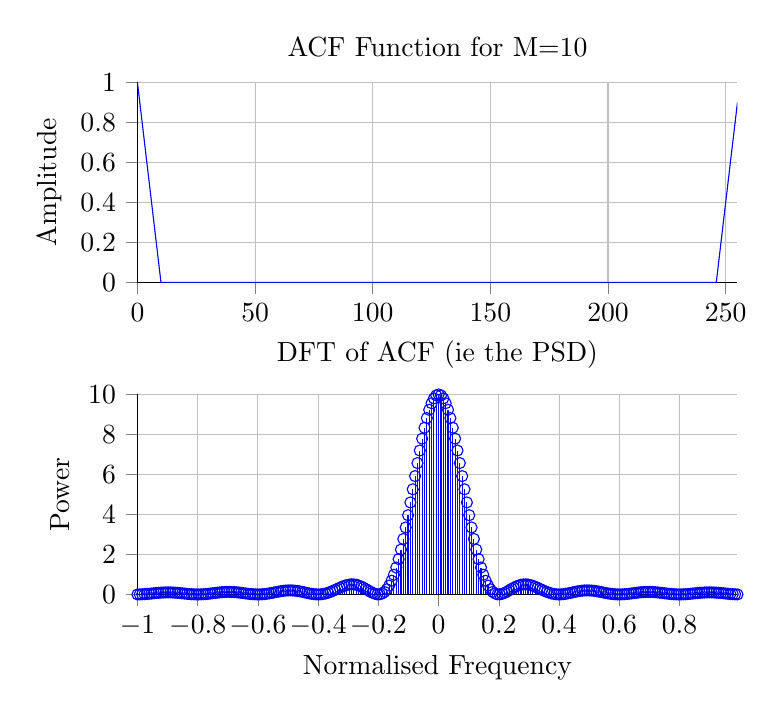
\begin{tikzpicture}

\begin{axis}[%
width=3in,
height=1in,
scale only axis,
every outer y axis line/.append style={black},
every y tick label/.append style={font=\color{black}},
every outer x axis line/.append style={black},
every x tick label/.append style={font=\color{black}},
tick align = outside,
xmin=0,
xmax=255,
xmajorgrids,
ymin=0,
ymax=1,
ylabel={Amplitude},
ymajorgrids,
name=plot1,
title={ACF Function for M=10},
axis x line*=bottom,
axis y line*=left
]
\addplot [color=blue,solid,forget plot]
  table[row sep=crcr]{0	1\\
1	0.9\\
2	0.8\\
3	0.7\\
4	0.6\\
5	0.5\\
6	0.4\\
7	0.3\\
8	0.2\\
9	0.1\\
10	0\\
11	0\\
12	0\\
13	0\\
14	0\\
15	0\\
16	0\\
17	0\\
18	0\\
19	0\\
20	0\\
21	0\\
22	0\\
23	0\\
24	0\\
25	0\\
26	0\\
27	0\\
28	0\\
29	0\\
30	0\\
31	0\\
32	0\\
33	0\\
34	0\\
35	0\\
36	0\\
37	0\\
38	0\\
39	0\\
40	0\\
41	0\\
42	0\\
43	0\\
44	0\\
45	0\\
46	0\\
47	0\\
48	0\\
49	0\\
50	0\\
51	0\\
52	0\\
53	0\\
54	0\\
55	0\\
56	0\\
57	0\\
58	0\\
59	0\\
60	0\\
61	0\\
62	0\\
63	0\\
64	0\\
65	0\\
66	0\\
67	0\\
68	0\\
69	0\\
70	0\\
71	0\\
72	0\\
73	0\\
74	0\\
75	0\\
76	0\\
77	0\\
78	0\\
79	0\\
80	0\\
81	0\\
82	0\\
83	0\\
84	0\\
85	0\\
86	0\\
87	0\\
88	0\\
89	0\\
90	0\\
91	0\\
92	0\\
93	0\\
94	0\\
95	0\\
96	0\\
97	0\\
98	0\\
99	0\\
100	0\\
101	0\\
102	0\\
103	0\\
104	0\\
105	0\\
106	0\\
107	0\\
108	0\\
109	0\\
110	0\\
111	0\\
112	0\\
113	0\\
114	0\\
115	0\\
116	0\\
117	0\\
118	0\\
119	0\\
120	0\\
121	0\\
122	0\\
123	0\\
124	0\\
125	0\\
126	0\\
127	0\\
128	0\\
129	0\\
130	0\\
131	0\\
132	0\\
133	0\\
134	0\\
135	0\\
136	0\\
137	0\\
138	0\\
139	0\\
140	0\\
141	0\\
142	0\\
143	0\\
144	0\\
145	0\\
146	0\\
147	0\\
148	0\\
149	0\\
150	0\\
151	0\\
152	0\\
153	0\\
154	0\\
155	0\\
156	0\\
157	0\\
158	0\\
159	0\\
160	0\\
161	0\\
162	0\\
163	0\\
164	0\\
165	0\\
166	0\\
167	0\\
168	0\\
169	0\\
170	0\\
171	0\\
172	0\\
173	0\\
174	0\\
175	0\\
176	0\\
177	0\\
178	0\\
179	0\\
180	0\\
181	0\\
182	0\\
183	0\\
184	0\\
185	0\\
186	0\\
187	0\\
188	0\\
189	0\\
190	0\\
191	0\\
192	0\\
193	0\\
194	0\\
195	0\\
196	0\\
197	0\\
198	0\\
199	0\\
200	0\\
201	0\\
202	0\\
203	0\\
204	0\\
205	0\\
206	0\\
207	0\\
208	0\\
209	0\\
210	0\\
211	0\\
212	0\\
213	0\\
214	0\\
215	0\\
216	0\\
217	0\\
218	0\\
219	0\\
220	0\\
221	0\\
222	0\\
223	0\\
224	0\\
225	0\\
226	0\\
227	0\\
228	0\\
229	0\\
230	0\\
231	0\\
232	0\\
233	0\\
234	0\\
235	0\\
236	0\\
237	0\\
238	0\\
239	0\\
240	0\\
241	0\\
242	0\\
243	0\\
244	0\\
245	0\\
246	0\\
247	0.1\\
248	0.2\\
249	0.3\\
250	0.4\\
251	0.5\\
252	0.6\\
253	0.7\\
254	0.8\\
255	0.9\\
};
\end{axis}

\begin{axis}[%
width=3in,
height=1in,
scale only axis,
every outer y axis line/.append style={black},
every y tick label/.append style={font=\color{black}},
every outer x axis line/.append style={black},
every x tick label/.append style={font=\color{black}},
tick align = outside,
xmin=-1,
xmax=0.9921875,
xlabel={Normalised Frequency},
xmajorgrids,
ymin=0,
ymax=10,
ylabel={Power},
ymajorgrids,
at=(plot1.below south west),
anchor=above north west,
title={DFT of ACF (ie the PSD)},
axis x line*=bottom,
axis y line*=left
]
\addplot[ycomb,color=blue,solid,mark=o,mark options={solid}] plot table[row sep=crcr] {-1	0\\
-0.9921875	0.00149866302491386\\
-0.984375	0.0059074947006259\\
-0.9765625	0.012970015141204\\
-0.96875	0.0222751187415957\\
-0.9609375	0.0332806503200211\\
-0.953125	0.0453445360505695\\
-0.9453125	0.0577617180575047\\
-0.9375	0.0698048115585563\\
-0.9296875	0.0807661883960882\\
-0.921875	0.0899991028308651\\
-0.9140625	0.0969555198419336\\
-0.90625	0.101218480923288\\
-0.8984375	0.10252713841752\\
-0.890625	0.100792991043844\\
-0.8828125	0.0961063388917006\\
-0.875	0.0887325194919155\\
-0.8671875	0.0790980580723636\\
-0.859375	0.067767433457453\\
-0.8515625	0.0554116949410044\\
-0.84375	0.0427706351605831\\
-0.8359375	0.0306106031051708\\
-0.828125	0.0196803081929335\\
-0.8203125	0.0106671050876996\\
-0.8125	0.00415625064032668\\
-0.8046875	0.00059548748189938\\
-0.796875	0.000267039330955426\\
-0.7890625	0.00326871426665155\\
-0.78125	0.00950532397470137\\
-0.7734375	0.0186910648558342\\
-0.765625	0.0303629008003442\\
-0.7578125	0.0439043700628398\\
-0.75	0.0585786437626903\\
-0.7421875	0.0735691240896914\\
-0.734375	0.0880254167858926\\
-0.7265625	0.101112171178689\\
-0.71875	0.112058072561143\\
-0.7109375	0.120202209794887\\
-0.703125	0.125035131685216\\
-0.6953125	0.126232146830954\\
-0.6875	0.123676802993121\\
-0.6796875	0.117472985502953\\
-0.671875	0.107944674853259\\
-0.6640625	0.0956230706728966\\
-0.65625	0.0812214878628928\\
-0.6484375	0.0655991234491216\\
-0.640625	0.0497154418776339\\
-0.6328125	0.0345774957627702\\
-0.625	0.0211829556901867\\
-0.6171875	0.0104619390598137\\
-0.609375	0.00322088346758906\\
-0.6015625	9.169220807273e-05\\
-0.59375	0.00148918451373481\\
-0.5859375	0.00757951684862983\\
-0.578125	0.0182617189161397\\
-0.5703125	0.0331638326818152\\
-0.5625	0.0516543859708854\\
-0.5546875	0.0728691116025978\\
-0.546875	0.0957519805036194\\
-0.5390625	0.119108797067965\\
-0.53125	0.141670851563638\\
-0.5234375	0.162165479784237\\
-0.515625	0.179389882121275\\
-0.5078125	0.19228423399171\\
-0.5	0.199999999999999\\
-0.4921875	0.201959458543945\\
-0.484375	0.197902754332944\\
-0.4765625	0.187919314930291\\
-0.46875	0.172461174438278\\
-0.4609375	0.152336612993292\\
-0.453125	0.12868350590966\\
-0.4453125	0.102922834786051\\
-0.4375	0.0766938930565673\\
-0.4296875	0.0517737658577898\\
-0.421875	0.0299846239968007\\
-0.4140625	0.0130931920410805\\
-0.40625	0.0027073840709031\\
-0.3984375	0.00017550805008823\\
-0.390625	0.00649359152292675\\
-0.3828125	0.0222262594605707\\
-0.375	0.047446194411337\\
-0.3671875	0.0816965379822724\\
-0.359375	0.123979672908331\\
-0.3515625	0.172774691215179\\
-0.34375	0.226084552494096\\
-0.3359375	0.281512523038993\\
-0.328125	0.336366024839946\\
-0.3203125	0.387784581025762\\
-0.3125	0.432887190608936\\
-0.3046875	0.46893326785671\\
-0.296875	0.493490302846846\\
-0.2890625	0.504600694249527\\
-0.28125	0.50093981674076\\
-0.2734375	0.48195734413734\\
-0.265625	0.44799417080793\\
-0.2578125	0.400367957500461\\
-0.25	0.34142135623731\\
-0.2421875	0.274528308965631\\
-0.234375	0.204055417688387\\
-0.2265625	0.135277187997608\\
-0.21875	0.0742458805676954\\
-0.2109375	0.0276186856481936\\
-0.203125	0.00244687886890835\\
-0.1953125	0.0059334369151034\\
-0.1875	0.0451672060621878\\
-0.1796875	0.126843049172281\\
-0.171875	0.256978381835627\\
-0.1640625	0.440637093586787\\
-0.15625	0.681671999231521\\
-0.1484375	0.982496659889203\\
-0.140625	1.34389665406111\\
-0.1328125	1.76488918595553\\
-0.125	2.24263833040656\\
-0.1171875	2.77243128752464\\
-0.109375	3.347718827625\\
-0.1015625	3.96022073246167\\
-0.09375	4.60009457594603\\
-0.0859375	5.25616373520178\\
-0.078125	5.91619818096614\\
-0.0703125	6.567239461824\\
-0.0625	7.19595945910942\\
-0.0546875	7.78904102692079\\
-0.046875	8.33356760837251\\
-0.0390625	8.81740838132219\\
-0.03125	9.22958546120914\\
-0.0234375	9.56061018134294\\
-0.015625	9.80277646679872\\
-0.0078125	9.95040078111115\\
0	10\\
0.0078125	9.95040078111115\\
0.015625	9.80277646679872\\
0.0234375	9.56061018134294\\
0.03125	9.22958546120914\\
0.0390625	8.81740838132219\\
0.046875	8.33356760837251\\
0.0546875	7.78904102692079\\
0.0625	7.19595945910942\\
0.0703125	6.567239461824\\
0.078125	5.91619818096614\\
0.0859375	5.25616373520178\\
0.09375	4.60009457594603\\
0.1015625	3.96022073246167\\
0.109375	3.347718827625\\
0.1171875	2.77243128752464\\
0.125	2.24263833040656\\
0.1328125	1.76488918595553\\
0.140625	1.34389665406111\\
0.1484375	0.982496659889203\\
0.15625	0.681671999231521\\
0.1640625	0.440637093586787\\
0.171875	0.256978381835627\\
0.1796875	0.126843049172281\\
0.1875	0.0451672060621878\\
0.1953125	0.0059334369151034\\
0.203125	0.00244687886890835\\
0.2109375	0.0276186856481936\\
0.21875	0.0742458805676954\\
0.2265625	0.135277187997608\\
0.234375	0.204055417688387\\
0.2421875	0.274528308965631\\
0.25	0.34142135623731\\
0.2578125	0.400367957500461\\
0.265625	0.44799417080793\\
0.2734375	0.48195734413734\\
0.28125	0.50093981674076\\
0.2890625	0.504600694249527\\
0.296875	0.493490302846846\\
0.3046875	0.46893326785671\\
0.3125	0.432887190608936\\
0.3203125	0.387784581025762\\
0.328125	0.336366024839946\\
0.3359375	0.281512523038993\\
0.34375	0.226084552494096\\
0.3515625	0.172774691215179\\
0.359375	0.123979672908331\\
0.3671875	0.0816965379822724\\
0.375	0.047446194411337\\
0.3828125	0.0222262594605707\\
0.390625	0.00649359152292675\\
0.3984375	0.00017550805008823\\
0.40625	0.0027073840709031\\
0.4140625	0.0130931920410805\\
0.421875	0.0299846239968007\\
0.4296875	0.0517737658577898\\
0.4375	0.0766938930565673\\
0.4453125	0.102922834786051\\
0.453125	0.12868350590966\\
0.4609375	0.152336612993292\\
0.46875	0.172461174438278\\
0.4765625	0.187919314930291\\
0.484375	0.197902754332944\\
0.4921875	0.201959458543945\\
0.5	0.199999999999999\\
0.5078125	0.19228423399171\\
0.515625	0.179389882121275\\
0.5234375	0.162165479784237\\
0.53125	0.141670851563638\\
0.5390625	0.119108797067965\\
0.546875	0.0957519805036194\\
0.5546875	0.0728691116025978\\
0.5625	0.0516543859708854\\
0.5703125	0.0331638326818152\\
0.578125	0.0182617189161397\\
0.5859375	0.00757951684862983\\
0.59375	0.00148918451373481\\
0.6015625	9.169220807273e-05\\
0.609375	0.00322088346758906\\
0.6171875	0.0104619390598137\\
0.625	0.0211829556901867\\
0.6328125	0.0345774957627702\\
0.640625	0.0497154418776339\\
0.6484375	0.0655991234491216\\
0.65625	0.0812214878628928\\
0.6640625	0.0956230706728966\\
0.671875	0.107944674853259\\
0.6796875	0.117472985502953\\
0.6875	0.123676802993121\\
0.6953125	0.126232146830954\\
0.703125	0.125035131685216\\
0.7109375	0.120202209794887\\
0.71875	0.112058072561143\\
0.7265625	0.101112171178689\\
0.734375	0.0880254167858926\\
0.7421875	0.0735691240896914\\
0.75	0.0585786437626903\\
0.7578125	0.0439043700628398\\
0.765625	0.0303629008003442\\
0.7734375	0.0186910648558342\\
0.78125	0.00950532397470137\\
0.7890625	0.00326871426665155\\
0.796875	0.000267039330955426\\
0.8046875	0.00059548748189938\\
0.8125	0.00415625064032668\\
0.8203125	0.0106671050876996\\
0.828125	0.0196803081929335\\
0.8359375	0.0306106031051708\\
0.84375	0.0427706351605831\\
0.8515625	0.0554116949410044\\
0.859375	0.067767433457453\\
0.8671875	0.0790980580723636\\
0.875	0.0887325194919155\\
0.8828125	0.0961063388917006\\
0.890625	0.100792991043844\\
0.8984375	0.10252713841752\\
0.90625	0.101218480923288\\
0.9140625	0.0969555198419336\\
0.921875	0.0899991028308651\\
0.9296875	0.0807661883960882\\
0.9375	0.0698048115585563\\
0.9453125	0.0577617180575047\\
0.953125	0.0453445360505695\\
0.9609375	0.0332806503200211\\
0.96875	0.0222751187415957\\
0.9765625	0.012970015141204\\
0.984375	0.0059074947006259\\
0.9921875	0.00149866302491386\\
};
\addplot [color=black,solid,forget plot]
  table[row sep=crcr]{-1	0\\
0.9921875	0\\
};
\end{axis}
\end{tikzpicture}%}
		\caption{\textit{ACF for $M=10$}}
		\label{fig:1_2_a_10}
	\end{subfigure}
	~ %add desired spacing between images, e. g. ~, \quad, \qquad, \hfill etc.
	\begin{subfigure}[b]{0.49\textwidth}
		\resizebox{\textwidth}{!}{% This file was created by matlab2tikz v0.4.7 (commit 6519689aa9dc12b7be17fdbac3b670671ea448dc) running on MATLAB 8.3.
% Copyright (c) 2008--2014, Nico Schlömer <nico.schloemer@gmail.com>
% All rights reserved.
% Minimal pgfplots version: 1.3
% 
% The latest updates can be retrieved from
%   http://www.mathworks.com/matlabcentral/fileexchange/22022-matlab2tikz
% where you can also make suggestions and rate matlab2tikz.
% 
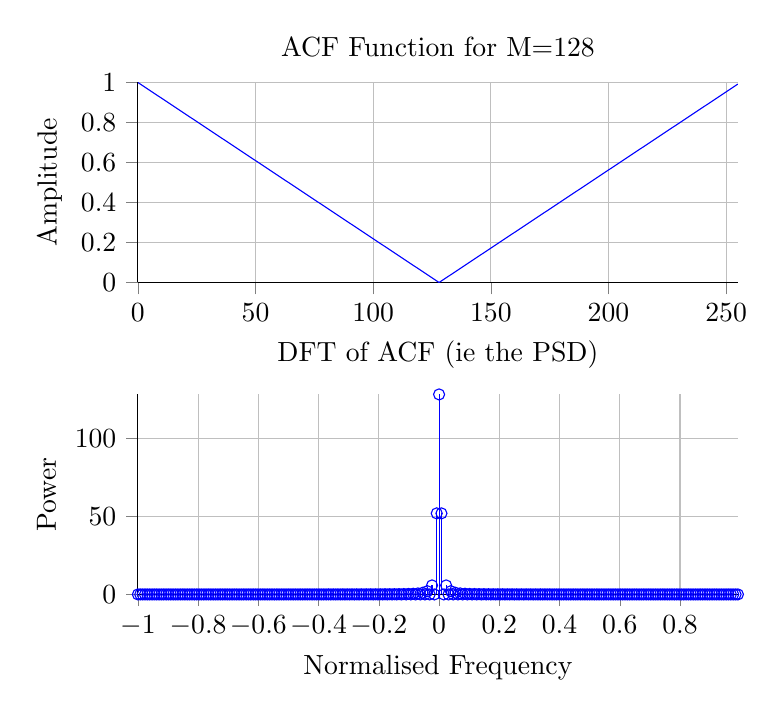
\begin{tikzpicture}

\begin{axis}[%
width=3in,
height=1in,
scale only axis,
every outer y axis line/.append style={black},
every y tick label/.append style={font=\color{black}},
every outer x axis line/.append style={black},
every x tick label/.append style={font=\color{black}},
tick align = outside,
xmin=0,
xmax=255,
xmajorgrids,
ymin=0,
ymax=1,
ylabel={Amplitude},
ymajorgrids,
name=plot1,
title={ACF Function for M=128},
axis x line*=bottom,
axis y line*=left
]
\addplot [color=blue,solid,forget plot]
  table[row sep=crcr]{0	1\\
1	0.9921875\\
2	0.984375\\
3	0.9765625\\
4	0.96875\\
5	0.9609375\\
6	0.953125\\
7	0.9453125\\
8	0.9375\\
9	0.9296875\\
10	0.921875\\
11	0.9140625\\
12	0.90625\\
13	0.8984375\\
14	0.890625\\
15	0.8828125\\
16	0.875\\
17	0.8671875\\
18	0.859375\\
19	0.8515625\\
20	0.84375\\
21	0.8359375\\
22	0.828125\\
23	0.8203125\\
24	0.8125\\
25	0.8046875\\
26	0.796875\\
27	0.7890625\\
28	0.78125\\
29	0.7734375\\
30	0.765625\\
31	0.7578125\\
32	0.75\\
33	0.7421875\\
34	0.734375\\
35	0.7265625\\
36	0.71875\\
37	0.7109375\\
38	0.703125\\
39	0.6953125\\
40	0.6875\\
41	0.6796875\\
42	0.671875\\
43	0.6640625\\
44	0.65625\\
45	0.6484375\\
46	0.640625\\
47	0.6328125\\
48	0.625\\
49	0.6171875\\
50	0.609375\\
51	0.6015625\\
52	0.59375\\
53	0.5859375\\
54	0.578125\\
55	0.5703125\\
56	0.5625\\
57	0.5546875\\
58	0.546875\\
59	0.5390625\\
60	0.53125\\
61	0.5234375\\
62	0.515625\\
63	0.5078125\\
64	0.5\\
65	0.4921875\\
66	0.484375\\
67	0.4765625\\
68	0.46875\\
69	0.4609375\\
70	0.453125\\
71	0.4453125\\
72	0.4375\\
73	0.4296875\\
74	0.421875\\
75	0.4140625\\
76	0.40625\\
77	0.3984375\\
78	0.390625\\
79	0.3828125\\
80	0.375\\
81	0.3671875\\
82	0.359375\\
83	0.3515625\\
84	0.34375\\
85	0.3359375\\
86	0.328125\\
87	0.3203125\\
88	0.3125\\
89	0.3046875\\
90	0.296875\\
91	0.2890625\\
92	0.28125\\
93	0.2734375\\
94	0.265625\\
95	0.2578125\\
96	0.25\\
97	0.2421875\\
98	0.234375\\
99	0.2265625\\
100	0.21875\\
101	0.2109375\\
102	0.203125\\
103	0.1953125\\
104	0.1875\\
105	0.1796875\\
106	0.171875\\
107	0.1640625\\
108	0.15625\\
109	0.1484375\\
110	0.140625\\
111	0.1328125\\
112	0.125\\
113	0.1171875\\
114	0.109375\\
115	0.1015625\\
116	0.09375\\
117	0.0859375\\
118	0.078125\\
119	0.0703125\\
120	0.0625\\
121	0.0546875\\
122	0.046875\\
123	0.0390625\\
124	0.03125\\
125	0.0234375\\
126	0.015625\\
127	0.0078125\\
128	0\\
129	0.0078125\\
130	0.015625\\
131	0.0234375\\
132	0.03125\\
133	0.0390625\\
134	0.046875\\
135	0.0546875\\
136	0.0625\\
137	0.0703125\\
138	0.078125\\
139	0.0859375\\
140	0.09375\\
141	0.1015625\\
142	0.109375\\
143	0.1171875\\
144	0.125\\
145	0.1328125\\
146	0.140625\\
147	0.1484375\\
148	0.15625\\
149	0.1640625\\
150	0.171875\\
151	0.1796875\\
152	0.1875\\
153	0.1953125\\
154	0.203125\\
155	0.2109375\\
156	0.21875\\
157	0.2265625\\
158	0.234375\\
159	0.2421875\\
160	0.25\\
161	0.2578125\\
162	0.265625\\
163	0.2734375\\
164	0.28125\\
165	0.2890625\\
166	0.296875\\
167	0.3046875\\
168	0.3125\\
169	0.3203125\\
170	0.328125\\
171	0.3359375\\
172	0.34375\\
173	0.3515625\\
174	0.359375\\
175	0.3671875\\
176	0.375\\
177	0.3828125\\
178	0.390625\\
179	0.3984375\\
180	0.40625\\
181	0.4140625\\
182	0.421875\\
183	0.4296875\\
184	0.4375\\
185	0.4453125\\
186	0.453125\\
187	0.4609375\\
188	0.46875\\
189	0.4765625\\
190	0.484375\\
191	0.4921875\\
192	0.5\\
193	0.5078125\\
194	0.515625\\
195	0.5234375\\
196	0.53125\\
197	0.5390625\\
198	0.546875\\
199	0.5546875\\
200	0.5625\\
201	0.5703125\\
202	0.578125\\
203	0.5859375\\
204	0.59375\\
205	0.6015625\\
206	0.609375\\
207	0.6171875\\
208	0.625\\
209	0.6328125\\
210	0.640625\\
211	0.6484375\\
212	0.65625\\
213	0.6640625\\
214	0.671875\\
215	0.6796875\\
216	0.6875\\
217	0.6953125\\
218	0.703125\\
219	0.7109375\\
220	0.71875\\
221	0.7265625\\
222	0.734375\\
223	0.7421875\\
224	0.75\\
225	0.7578125\\
226	0.765625\\
227	0.7734375\\
228	0.78125\\
229	0.7890625\\
230	0.796875\\
231	0.8046875\\
232	0.8125\\
233	0.8203125\\
234	0.828125\\
235	0.8359375\\
236	0.84375\\
237	0.8515625\\
238	0.859375\\
239	0.8671875\\
240	0.875\\
241	0.8828125\\
242	0.890625\\
243	0.8984375\\
244	0.90625\\
245	0.9140625\\
246	0.921875\\
247	0.9296875\\
248	0.9375\\
249	0.9453125\\
250	0.953125\\
251	0.9609375\\
252	0.96875\\
253	0.9765625\\
254	0.984375\\
255	0.9921875\\
};
\end{axis}

\begin{axis}[%
width=3in,
height=1in,
scale only axis,
every outer y axis line/.append style={black},
every y tick label/.append style={font=\color{black}},
every outer x axis line/.append style={black},
every x tick label/.append style={font=\color{black}},
tick align = outside,
xmin=-1,
xmax=0.9921875,
xlabel={Normalised Frequency},
xmajorgrids,
ymin=0,
ymax=128,
ylabel={Power},
ymajorgrids,
at=(plot1.below south west),
anchor=above north west,
title={DFT of ACF (ie the PSD)},
axis x line*=bottom,
axis y line*=left
]
\addplot[ycomb,color=blue,solid,mark=o,mark options={solid}] plot table[row sep=crcr] {-1	0\\
-0.9921875	0.007813676666661\\
-0.984375	0\\
-0.9765625	0.00782309851216301\\
-0.96875	0\\
-0.9609375	0.00784198769858219\\
-0.953125	0\\
-0.9453125	0.00787043568435053\\
-0.9375	0\\
-0.9296875	0.00790858083434676\\
-0.921875	0\\
-0.9140625	0.00795660985595675\\
-0.90625	0\\
-0.8984375	0.00801475975343256\\
-0.890625	0\\
-0.8828125	0.00808332033591525\\
-0.875	0\\
-0.8671875	0.00816263732511155\\
-0.859375	0\\
-0.8515625	0.0082531161205426\\
-0.84375	0\\
-0.8359375	0.00835522629390431\\
-0.828125	0\\
-0.8203125	0.00846950689979744\\
-0.8125	0\\
-0.8046875	0.00859657270843165\\
-0.796875	0\\
-0.7890625	0.00873712148754993\\
-0.78125	0\\
-0.7734375	0.00889194248655429\\
-0.765625	0\\
-0.7578125	0.00906192630655518\\
-0.75	0\\
-0.7421875	0.00924807637713809\\
-0.734375	0\\
-0.7265625	0.0094515223054852\\
-0.71875	0\\
-0.7109375	0.00967353541815228\\
-0.703125	0\\
-0.6953125	0.00991554688260718\\
-0.6875	0\\
-0.6796875	0.0101791688778967\\
-0.671875	0\\
-0.6640625	0.0104662193854375\\
-0.65625	0\\
-0.6484375	0.010778751297234\\
-0.640625	0\\
-0.6328125	0.0111190866965538\\
-0.625	0\\
-0.6171875	0.0114898573641483\\
-0.609375	0\\
-0.6015625	0.0118940528131687\\
-0.59375	0\\
-0.5859375	0.0123350774734022\\
-0.578125	0\\
-0.5703125	0.0128168190510498\\
-0.5625	0\\
-0.5546875	0.0133437306115424\\
-0.546875	0\\
-0.5390625	0.013920929607362\\
-0.53125	0\\
-0.5234375	0.0145543179514134\\
-0.515625	0\\
-0.5078125	0.0152507283894516\\
-0.5	0\\
-0.4921875	0.0160181039495291\\
-0.484375	0\\
-0.4765625	0.0168657192785184\\
-0.46875	0\\
-0.4609375	0.0178044554080542\\
-0.453125	0\\
-0.4453125	0.0188471431990445\\
-0.4375	0\\
-0.4296875	0.0200089957924109\\
-0.421875	0\\
-0.4140625	0.0213081574229965\\
-0.40625	0\\
-0.3984375	0.0227664057912161\\
-0.390625	0\\
-0.3828125	0.024410059118146\\
-0.375	0\\
-0.3671875	0.02627115898923\\
-0.359375	0\\
-0.3515625	0.0283890291386168\\
-0.34375	0\\
-0.3359375	0.0308123531815138\\
-0.328125	0\\
-0.3203125	0.0336019785451553\\
-0.3125	0\\
-0.3046875	0.0368347518360298\\
-0.296875	0\\
-0.2890625	0.0406088431833023\\
-0.28125	0\\
-0.2734375	0.045051258768406\\
-0.265625	0\\
-0.2578125	0.0503286330473229\\
-0.25	0\\
-0.2421875	0.0566630451900175\\
-0.234375	0\\
-0.2265625	0.0643557220894265\\
-0.21875	0\\
-0.2109375	0.0738234645642303\\
-0.203125	0\\
-0.1953125	0.0856562453486069\\
-0.1875	0\\
-0.1796875	0.100711305581392\\
-0.171875	0\\
-0.1640625	0.120272789717887\\
-0.15625	0\\
-0.1484375	0.146334795041807\\
-0.140625	0\\
-0.1328125	0.182130265837731\\
-0.125	0\\
-0.1171875	0.233183892600793\\
-0.109375	0\\
-0.1015625	0.309578695271768\\
-0.09375	0\\
-0.0859375	0.431344643896604\\
-0.078125	0\\
-0.0703125	0.643060483275948\\
-0.0625	0\\
-0.0546875	1.06131099466455\\
-0.046875	0\\
-0.0390625	2.07766396974844\\
-0.03125	0\\
-0.0234375	5.76665443106735\\
-0.015625	0\\
-0.0078125	51.879050269982\\
0	128\\
0.0078125	51.879050269982\\
0.015625	0\\
0.0234375	5.76665443106735\\
0.03125	0\\
0.0390625	2.07766396974844\\
0.046875	0\\
0.0546875	1.06131099466455\\
0.0625	0\\
0.0703125	0.643060483275948\\
0.078125	0\\
0.0859375	0.431344643896604\\
0.09375	0\\
0.1015625	0.309578695271768\\
0.109375	0\\
0.1171875	0.233183892600793\\
0.125	0\\
0.1328125	0.182130265837731\\
0.140625	0\\
0.1484375	0.146334795041807\\
0.15625	0\\
0.1640625	0.120272789717887\\
0.171875	0\\
0.1796875	0.100711305581392\\
0.1875	0\\
0.1953125	0.0856562453486069\\
0.203125	0\\
0.2109375	0.0738234645642303\\
0.21875	0\\
0.2265625	0.0643557220894265\\
0.234375	0\\
0.2421875	0.0566630451900175\\
0.25	0\\
0.2578125	0.0503286330473229\\
0.265625	0\\
0.2734375	0.045051258768406\\
0.28125	0\\
0.2890625	0.0406088431833023\\
0.296875	0\\
0.3046875	0.0368347518360298\\
0.3125	0\\
0.3203125	0.0336019785451553\\
0.328125	0\\
0.3359375	0.0308123531815138\\
0.34375	0\\
0.3515625	0.0283890291386168\\
0.359375	0\\
0.3671875	0.02627115898923\\
0.375	0\\
0.3828125	0.024410059118146\\
0.390625	0\\
0.3984375	0.0227664057912161\\
0.40625	0\\
0.4140625	0.0213081574229965\\
0.421875	0\\
0.4296875	0.0200089957924109\\
0.4375	0\\
0.4453125	0.0188471431990445\\
0.453125	0\\
0.4609375	0.0178044554080542\\
0.46875	0\\
0.4765625	0.0168657192785184\\
0.484375	0\\
0.4921875	0.0160181039495291\\
0.5	0\\
0.5078125	0.0152507283894516\\
0.515625	0\\
0.5234375	0.0145543179514134\\
0.53125	0\\
0.5390625	0.013920929607362\\
0.546875	0\\
0.5546875	0.0133437306115424\\
0.5625	0\\
0.5703125	0.0128168190510498\\
0.578125	0\\
0.5859375	0.0123350774734022\\
0.59375	0\\
0.6015625	0.0118940528131687\\
0.609375	0\\
0.6171875	0.0114898573641483\\
0.625	0\\
0.6328125	0.0111190866965538\\
0.640625	0\\
0.6484375	0.010778751297234\\
0.65625	0\\
0.6640625	0.0104662193854375\\
0.671875	0\\
0.6796875	0.0101791688778967\\
0.6875	0\\
0.6953125	0.00991554688260718\\
0.703125	0\\
0.7109375	0.00967353541815228\\
0.71875	0\\
0.7265625	0.0094515223054852\\
0.734375	0\\
0.7421875	0.00924807637713809\\
0.75	0\\
0.7578125	0.00906192630655518\\
0.765625	0\\
0.7734375	0.00889194248655429\\
0.78125	0\\
0.7890625	0.00873712148754993\\
0.796875	0\\
0.8046875	0.00859657270843165\\
0.8125	0\\
0.8203125	0.00846950689979744\\
0.828125	0\\
0.8359375	0.00835522629390431\\
0.84375	0\\
0.8515625	0.0082531161205426\\
0.859375	0\\
0.8671875	0.00816263732511155\\
0.875	0\\
0.8828125	0.00808332033591525\\
0.890625	0\\
0.8984375	0.00801475975343256\\
0.90625	0\\
0.9140625	0.00795660985595675\\
0.921875	0\\
0.9296875	0.00790858083434676\\
0.9375	0\\
0.9453125	0.00787043568435053\\
0.953125	0\\
0.9609375	0.00784198769858219\\
0.96875	0\\
0.9765625	0.00782309851216301\\
0.984375	0\\
0.9921875	0.007813676666661\\
};
\addplot [color=black,solid,forget plot]
  table[row sep=crcr]{-1	0\\
0.9921875	0\\
};
\end{axis}
\end{tikzpicture}%}
		\caption{\textit{ACF for $M=128$}}
		\label{fig:1_2_a_128}
	\end{subfigure}
	\label{fig:1_2_a}
	\caption{\textit{Autocorrelation Functions and their DFTs}}
\end{figure}

\subsubsection{The Real Component of the PSD}
The DFTs in Figure \ref{fig:1_2_a} show the real components of the DFT of the ACF. 

\subsubsection{Erroneous Spectral Values}

By taking the incorrect wrap around, as observed for the modified ACF function, visible in Figure \ref{fig:1_2_c}, we observe negative power from the DFT of the ACF (which, as demonstrated earlier, represents the PSD). This is clearly incorrect (in this context, we cannot have negative power), and demonstrates the need to be careful when representing the ACF in a programming environment such as \texttt{MATLAB}. Effectively, we must wrap around the information which would have been stored in negative indices round to the last samples of the signal.

\begin{figure}[h]
	\centering
	\begin{subfigure}[b]{0.49\textwidth}
		\resizebox{\textwidth}{!}{% This file was created by matlab2tikz v0.4.7 (commit 6519689aa9dc12b7be17fdbac3b670671ea448dc) running on MATLAB 8.3.
% Copyright (c) 2008--2014, Nico Schlömer <nico.schloemer@gmail.com>
% All rights reserved.
% Minimal pgfplots version: 1.3
% 
% The latest updates can be retrieved from
%   http://www.mathworks.com/matlabcentral/fileexchange/22022-matlab2tikz
% where you can also make suggestions and rate matlab2tikz.
% 
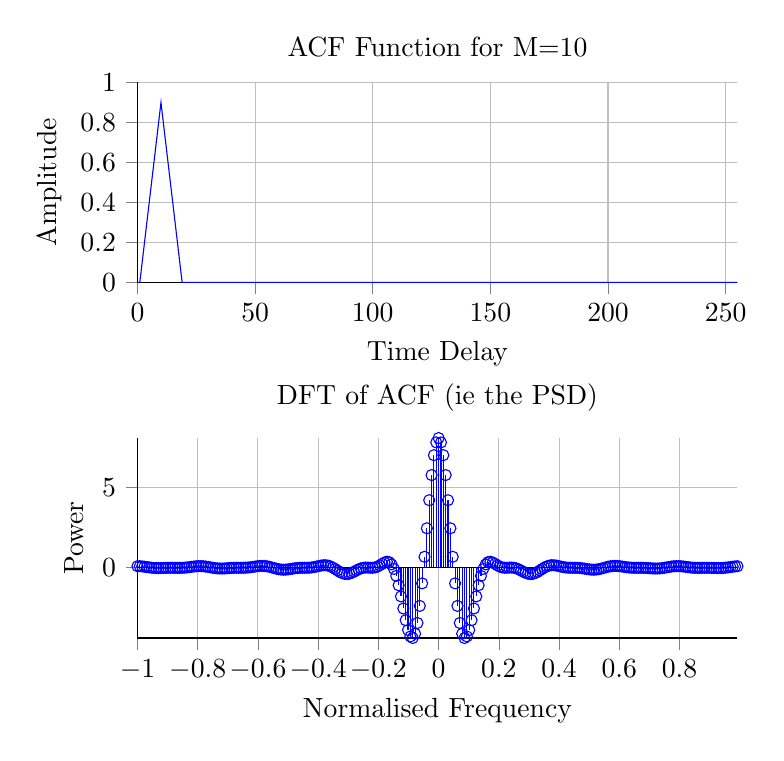
\begin{tikzpicture}

\begin{axis}[%
width=3in,
height=1in,
scale only axis,
every outer y axis line/.append style={black},
every y tick label/.append style={font=\color{black}},
every outer x axis line/.append style={black},
every x tick label/.append style={font=\color{black}},
tick align = outside,
xmin=0,
xmax=255,
xlabel={Time Delay},
xmajorgrids,
ymin=0,
ymax=1,
ylabel={Amplitude},
ymajorgrids,
name=plot1,
title={ACF Function for M=10},
axis x line*=bottom,
axis y line*=left
]
\addplot [color=blue,solid,forget plot]
  table[row sep=crcr]{0	0\\
1	0\\
2	0.1\\
3	0.2\\
4	0.3\\
5	0.4\\
6	0.5\\
7	0.6\\
8	0.7\\
9	0.8\\
10	0.9\\
11	0.8\\
12	0.7\\
13	0.6\\
14	0.5\\
15	0.4\\
16	0.3\\
17	0.2\\
18	0.1\\
19	0\\
20	0\\
21	0\\
22	0\\
23	0\\
24	0\\
25	0\\
26	0\\
27	0\\
28	0\\
29	0\\
30	0\\
31	0\\
32	0\\
33	0\\
34	0\\
35	0\\
36	0\\
37	0\\
38	0\\
39	0\\
40	0\\
41	0\\
42	0\\
43	0\\
44	0\\
45	0\\
46	0\\
47	0\\
48	0\\
49	0\\
50	0\\
51	0\\
52	0\\
53	0\\
54	0\\
55	0\\
56	0\\
57	0\\
58	0\\
59	0\\
60	0\\
61	0\\
62	0\\
63	0\\
64	0\\
65	0\\
66	0\\
67	0\\
68	0\\
69	0\\
70	0\\
71	0\\
72	0\\
73	0\\
74	0\\
75	0\\
76	0\\
77	0\\
78	0\\
79	0\\
80	0\\
81	0\\
82	0\\
83	0\\
84	0\\
85	0\\
86	0\\
87	0\\
88	0\\
89	0\\
90	0\\
91	0\\
92	0\\
93	0\\
94	0\\
95	0\\
96	0\\
97	0\\
98	0\\
99	0\\
100	0\\
101	0\\
102	0\\
103	0\\
104	0\\
105	0\\
106	0\\
107	0\\
108	0\\
109	0\\
110	0\\
111	0\\
112	0\\
113	0\\
114	0\\
115	0\\
116	0\\
117	0\\
118	0\\
119	0\\
120	0\\
121	0\\
122	0\\
123	0\\
124	0\\
125	0\\
126	0\\
127	0\\
128	0\\
129	0\\
130	0\\
131	0\\
132	0\\
133	0\\
134	0\\
135	0\\
136	0\\
137	0\\
138	0\\
139	0\\
140	0\\
141	0\\
142	0\\
143	0\\
144	0\\
145	0\\
146	0\\
147	0\\
148	0\\
149	0\\
150	0\\
151	0\\
152	0\\
153	0\\
154	0\\
155	0\\
156	0\\
157	0\\
158	0\\
159	0\\
160	0\\
161	0\\
162	0\\
163	0\\
164	0\\
165	0\\
166	0\\
167	0\\
168	0\\
169	0\\
170	0\\
171	0\\
172	0\\
173	0\\
174	0\\
175	0\\
176	0\\
177	0\\
178	0\\
179	0\\
180	0\\
181	0\\
182	0\\
183	0\\
184	0\\
185	0\\
186	0\\
187	0\\
188	0\\
189	0\\
190	0\\
191	0\\
192	0\\
193	0\\
194	0\\
195	0\\
196	0\\
197	0\\
198	0\\
199	0\\
200	0\\
201	0\\
202	0\\
203	0\\
204	0\\
205	0\\
206	0\\
207	0\\
208	0\\
209	0\\
210	0\\
211	0\\
212	0\\
213	0\\
214	0\\
215	0\\
216	0\\
217	0\\
218	0\\
219	0\\
220	0\\
221	0\\
222	0\\
223	0\\
224	0\\
225	0\\
226	0\\
227	0\\
228	0\\
229	0\\
230	0\\
231	0\\
232	0\\
233	0\\
234	0\\
235	0\\
236	0\\
237	0\\
238	0\\
239	0\\
240	0\\
241	0\\
242	0\\
243	0\\
244	0\\
245	0\\
246	0\\
247	0\\
248	0\\
249	0\\
250	0\\
251	0\\
252	0\\
253	0\\
254	0\\
255	0\\
};
\end{axis}

\begin{axis}[%
width=3in,
height=1in,
scale only axis,
every outer y axis line/.append style={black},
every y tick label/.append style={font=\color{black}},
every outer x axis line/.append style={black},
every x tick label/.append style={font=\color{black}},
tick align = outside,
xmin=-1,
xmax=0.9921875,
xlabel={Normalised Frequency},
xmajorgrids,
ymin=-4.38521661963401,
ymax=8.1,
ylabel={Power},
ymajorgrids,
at=(plot1.below south west),
anchor=above north west,
title={DFT of ACF (ie the PSD)},
axis x line*=bottom,
axis y line*=left
]
\addplot[ycomb,color=blue,solid,mark=o,mark options={solid}] plot table[row sep=crcr] {-1	0.0999999999999996\\
-0.9921875	0.0958390731255192\\
-0.984375	0.0840090285118595\\
-0.9765625	0.0663437455300278\\
-0.96875	0.0455105858414906\\
-0.9609375	0.0245101312130366\\
-0.953125	0.00612481406803833\\
-0.9453125	-0.0075723121718807\\
-0.9375	-0.0155506809022752\\
-0.9296875	-0.0179327303545069\\
-0.921875	-0.0158641475064105\\
-0.9140625	-0.0111764577971029\\
-0.90625	-0.00591790581149398\\
-0.8984375	-0.0018558490843863\\
-0.890625	-5.93690642463063e-05\\
-0.8828125	-0.00065327648076452\\
-0.875	-0.00279774787551768\\
-0.8671875	-0.00489915736046509\\
-0.859375	-0.00500745477580611\\
-0.8515625	-0.00131428200762107\\
-0.84375	0.00735729987631287\\
-0.8359375	0.0211809499478115\\
-0.828125	0.0391595471924268\\
-0.8203125	0.0592067552646219\\
-0.8125	0.0784702891064521\\
-0.8046875	0.0938379711081268\\
-0.796875	0.102527474331042\\
-0.7890625	0.102640442589219\\
-0.78125	0.0935660287852061\\
-0.7734375	0.076147321729537\\
-0.765625	0.0525711218081756\\
-0.7578125	0.0259975995094763\\
-0.75	0\\
-0.7421875	-0.0220754689192317\\
-0.734375	-0.037701662424617\\
-0.7265625	-0.0455950473151461\\
-0.71875	-0.0458868343317684\\
-0.7109375	-0.0400065778754285\\
-0.703125	-0.0303038001175696\\
-0.6953125	-0.0194883617254355\\
-0.6875	-0.0100093054299212\\
-0.6796875	-0.00350623922422307\\
-0.671875	-0.000453492962474746\\
-0.6640625	-7.75993335596775e-05\\
-0.65625	-0.000570921734272131\\
-0.6484375	0.000439740576027109\\
-0.640625	0.00526760188209421\\
-0.6328125	0.0155189127079421\\
-0.625	0.0315696797181403\\
-0.6171875	0.0522900435465032\\
-0.609375	0.0750918387127709\\
-0.6015625	0.0963084823040084\\
-0.59375	0.111845415709581\\
-0.5859375	0.117978645189596\\
-0.578125	0.112141632984481\\
-0.5703125	0.0935355803574195\\
-0.5625	0.0634273155692684\\
-0.5546875	0.0250577545906094\\
-0.546875	-0.0168389027848674\\
-0.5390625	-0.0568248388367422\\
-0.53125	-0.089710059573868\\
-0.5234375	-0.111479803388507\\
-0.515625	-0.120010483950155\\
-0.5078125	-0.115423984007487\\
-0.5	-0.1\\
-0.4921875	-0.0776553786565126\\
-0.484375	-0.0530901434457669\\
-0.4765625	-0.0307732816296473\\
-0.46875	-0.0139812673784461\\
-0.4609375	-0.00409891603048648\\
-0.453125	-0.000344258264615593\\
-0.4453125	5.33057226234646e-06\\
-0.4375	0.000913537884852336\\
-0.4296875	0.00654440645672252\\
-0.421875	0.0200949342765\\
-0.4140625	0.0427565104575643\\
-0.40625	0.0730498952296205\\
-0.3984375	0.106714917704939\\
-0.390625	0.137229916273016\\
-0.3828125	0.15690669039228\\
-0.375	0.158379813943026\\
-0.3671875	0.136211094449971\\
-0.359375	0.0882829822991724\\
-0.3515625	0.0166720036926049\\
-0.34375	-0.0722243215019041\\
-0.3359375	-0.168398474374917\\
-0.328125	-0.259709270603403\\
-0.3203125	-0.333889554273882\\
-0.3125	-0.38072546326478\\
-0.3046875	-0.393985406053245\\
-0.296875	-0.372695852957135\\
-0.2890625	-0.321463305181\\
-0.28125	-0.249713106030583\\
-0.2734375	-0.169926996134726\\
-0.265625	-0.0951732324203023\\
-0.2578125	-0.0363932745677173\\
-0.25	0\\
-0.2421875	0.0136707560632411\\
-0.234375	0.0106373505612004\\
-0.2265625	0.00208015646871114\\
-0.21875	0.00176384926368353\\
-0.2109375	0.0224524639431927\\
-0.203125	0.0719470188241617\\
-0.1953125	0.149531578379678\\
-0.1875	0.243635329486726\\
-0.1796875	0.331388296753799\\
-0.171875	0.380475973832865\\
-0.1640625	0.353319502958626\\
-0.15625	0.213181528231025\\
-0.1484375	-0.0686046011597217\\
-0.140625	-0.505389416977674\\
-0.1328125	-1.08919766799593\\
-0.125	-1.78715174578565\\
-0.1171875	-2.54126333149054\\
-0.109375	-3.27208520556482\\
-0.1015625	-3.88615000324389\\
-0.09375	-4.28651896464354\\
-0.0859375	-4.38521661963401\\
-0.078125	-4.1159286733062\\
-0.0703125	-3.44516319629736\\
-0.0625	-2.38016102245032\\
-0.0546875	-0.972191629436885\\
-0.046875	0.685554453297734\\
-0.0390625	2.46554366741177\\
-0.03125	4.21824877806895\\
-0.0234375	5.78787397131022\\
-0.015625	7.02953967827053\\
-0.0078125	7.82574912573789\\
0	8.1\\
0.0078125	7.82574912573789\\
0.015625	7.02953967827053\\
0.0234375	5.78787397131022\\
0.03125	4.21824877806895\\
0.0390625	2.46554366741177\\
0.046875	0.685554453297734\\
0.0546875	-0.972191629436885\\
0.0625	-2.38016102245032\\
0.0703125	-3.44516319629736\\
0.078125	-4.1159286733062\\
0.0859375	-4.38521661963401\\
0.09375	-4.28651896464354\\
0.1015625	-3.88615000324389\\
0.109375	-3.27208520556482\\
0.1171875	-2.54126333149054\\
0.125	-1.78715174578565\\
0.1328125	-1.08919766799593\\
0.140625	-0.505389416977674\\
0.1484375	-0.0686046011597217\\
0.15625	0.213181528231025\\
0.1640625	0.353319502958626\\
0.171875	0.380475973832865\\
0.1796875	0.331388296753799\\
0.1875	0.243635329486726\\
0.1953125	0.149531578379678\\
0.203125	0.0719470188241617\\
0.2109375	0.0224524639431927\\
0.21875	0.00176384926368353\\
0.2265625	0.00208015646871114\\
0.234375	0.0106373505612004\\
0.2421875	0.0136707560632411\\
0.25	0\\
0.2578125	-0.0363932745677173\\
0.265625	-0.0951732324203023\\
0.2734375	-0.169926996134726\\
0.28125	-0.249713106030583\\
0.2890625	-0.321463305181\\
0.296875	-0.372695852957135\\
0.3046875	-0.393985406053245\\
0.3125	-0.38072546326478\\
0.3203125	-0.333889554273882\\
0.328125	-0.259709270603403\\
0.3359375	-0.168398474374917\\
0.34375	-0.0722243215019041\\
0.3515625	0.0166720036926049\\
0.359375	0.0882829822991724\\
0.3671875	0.136211094449971\\
0.375	0.158379813943026\\
0.3828125	0.15690669039228\\
0.390625	0.137229916273016\\
0.3984375	0.106714917704939\\
0.40625	0.0730498952296205\\
0.4140625	0.0427565104575643\\
0.421875	0.0200949342765\\
0.4296875	0.00654440645672252\\
0.4375	0.000913537884852336\\
0.4453125	5.33057226234646e-06\\
0.453125	-0.000344258264615593\\
0.4609375	-0.00409891603048648\\
0.46875	-0.0139812673784461\\
0.4765625	-0.0307732816296473\\
0.484375	-0.0530901434457669\\
0.4921875	-0.0776553786565126\\
0.5	-0.1\\
0.5078125	-0.115423984007487\\
0.515625	-0.120010483950155\\
0.5234375	-0.111479803388507\\
0.53125	-0.089710059573868\\
0.5390625	-0.0568248388367422\\
0.546875	-0.0168389027848674\\
0.5546875	0.0250577545906094\\
0.5625	0.0634273155692684\\
0.5703125	0.0935355803574195\\
0.578125	0.112141632984481\\
0.5859375	0.117978645189596\\
0.59375	0.111845415709581\\
0.6015625	0.0963084823040084\\
0.609375	0.0750918387127709\\
0.6171875	0.0522900435465032\\
0.625	0.0315696797181403\\
0.6328125	0.0155189127079421\\
0.640625	0.00526760188209421\\
0.6484375	0.000439740576027109\\
0.65625	-0.000570921734272131\\
0.6640625	-7.75993335596775e-05\\
0.671875	-0.000453492962474746\\
0.6796875	-0.00350623922422307\\
0.6875	-0.0100093054299212\\
0.6953125	-0.0194883617254355\\
0.703125	-0.0303038001175696\\
0.7109375	-0.0400065778754285\\
0.71875	-0.0458868343317684\\
0.7265625	-0.0455950473151461\\
0.734375	-0.037701662424617\\
0.7421875	-0.0220754689192317\\
0.75	0\\
0.7578125	0.0259975995094763\\
0.765625	0.0525711218081756\\
0.7734375	0.076147321729537\\
0.78125	0.0935660287852061\\
0.7890625	0.102640442589219\\
0.796875	0.102527474331042\\
0.8046875	0.0938379711081268\\
0.8125	0.0784702891064521\\
0.8203125	0.0592067552646219\\
0.828125	0.0391595471924268\\
0.8359375	0.0211809499478115\\
0.84375	0.00735729987631287\\
0.8515625	-0.00131428200762107\\
0.859375	-0.00500745477580611\\
0.8671875	-0.00489915736046509\\
0.875	-0.00279774787551768\\
0.8828125	-0.00065327648076452\\
0.890625	-5.93690642463063e-05\\
0.8984375	-0.0018558490843863\\
0.90625	-0.00591790581149398\\
0.9140625	-0.0111764577971029\\
0.921875	-0.0158641475064105\\
0.9296875	-0.0179327303545069\\
0.9375	-0.0155506809022752\\
0.9453125	-0.0075723121718807\\
0.953125	0.00612481406803833\\
0.9609375	0.0245101312130366\\
0.96875	0.0455105858414906\\
0.9765625	0.0663437455300278\\
0.984375	0.0840090285118595\\
0.9921875	0.0958390731255192\\
};
\addplot [color=black,solid,forget plot]
  table[row sep=crcr]{-1	0\\
0.9921875	0\\
};
\end{axis}
\end{tikzpicture}%}
		\caption{\textit{1 Tree}}
		\label{fig:1_2_c_10}
	\end{subfigure}
	~ %add desired spacing between images, e. g. ~, \quad, \qquad, \hfill etc.
	\begin{subfigure}[b]{0.49\textwidth}
		\resizebox{\textwidth}{!}{% This file was created by matlab2tikz v0.4.7 (commit 6519689aa9dc12b7be17fdbac3b670671ea448dc) running on MATLAB 8.3.
% Copyright (c) 2008--2014, Nico Schlömer <nico.schloemer@gmail.com>
% All rights reserved.
% Minimal pgfplots version: 1.3
% 
% The latest updates can be retrieved from
%   http://www.mathworks.com/matlabcentral/fileexchange/22022-matlab2tikz
% where you can also make suggestions and rate matlab2tikz.
% 
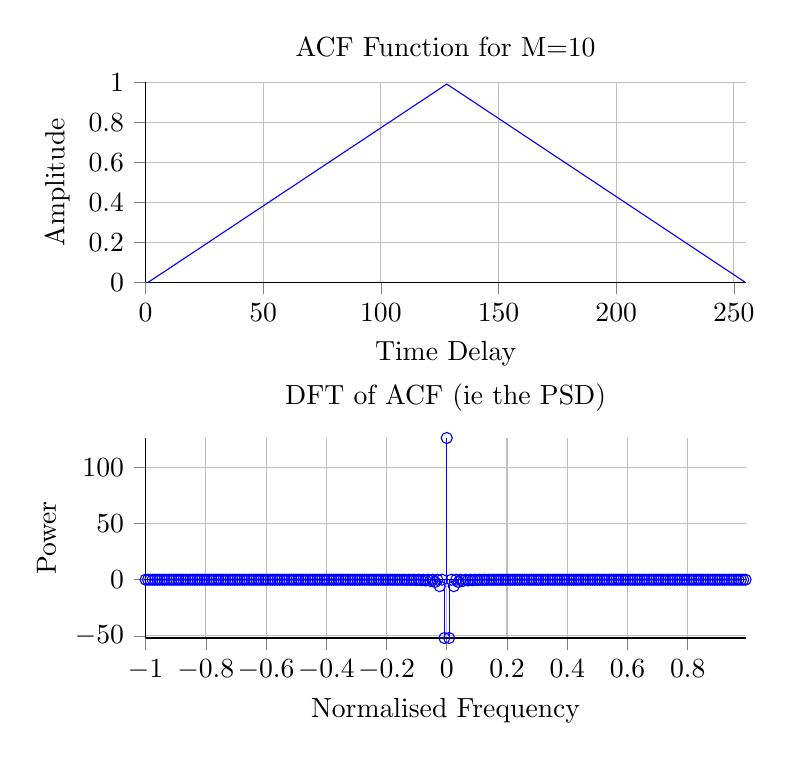
\begin{tikzpicture}

\begin{axis}[%
width=3in,
height=1in,
scale only axis,
every outer y axis line/.append style={black},
every y tick label/.append style={font=\color{black}},
every outer x axis line/.append style={black},
every x tick label/.append style={font=\color{black}},
tick align = outside,
xmin=0,
xmax=255,
xlabel={Time Delay},
xmajorgrids,
ymin=0,
ymax=1,
ylabel={Amplitude},
ymajorgrids,
name=plot1,
title={ACF Function for M=10},
axis x line*=bottom,
axis y line*=left
]
\addplot [color=blue,solid,forget plot]
  table[row sep=crcr]{0	0\\
1	0\\
2	0.0078125\\
3	0.015625\\
4	0.0234375\\
5	0.03125\\
6	0.0390625\\
7	0.046875\\
8	0.0546875\\
9	0.0625\\
10	0.0703125\\
11	0.078125\\
12	0.0859375\\
13	0.09375\\
14	0.1015625\\
15	0.109375\\
16	0.1171875\\
17	0.125\\
18	0.1328125\\
19	0.140625\\
20	0.1484375\\
21	0.15625\\
22	0.1640625\\
23	0.171875\\
24	0.1796875\\
25	0.1875\\
26	0.1953125\\
27	0.203125\\
28	0.2109375\\
29	0.21875\\
30	0.2265625\\
31	0.234375\\
32	0.2421875\\
33	0.25\\
34	0.2578125\\
35	0.265625\\
36	0.2734375\\
37	0.28125\\
38	0.2890625\\
39	0.296875\\
40	0.3046875\\
41	0.3125\\
42	0.3203125\\
43	0.328125\\
44	0.3359375\\
45	0.34375\\
46	0.3515625\\
47	0.359375\\
48	0.3671875\\
49	0.375\\
50	0.3828125\\
51	0.390625\\
52	0.3984375\\
53	0.40625\\
54	0.4140625\\
55	0.421875\\
56	0.4296875\\
57	0.4375\\
58	0.4453125\\
59	0.453125\\
60	0.4609375\\
61	0.46875\\
62	0.4765625\\
63	0.484375\\
64	0.4921875\\
65	0.5\\
66	0.5078125\\
67	0.515625\\
68	0.5234375\\
69	0.53125\\
70	0.5390625\\
71	0.546875\\
72	0.5546875\\
73	0.5625\\
74	0.5703125\\
75	0.578125\\
76	0.5859375\\
77	0.59375\\
78	0.6015625\\
79	0.609375\\
80	0.6171875\\
81	0.625\\
82	0.6328125\\
83	0.640625\\
84	0.6484375\\
85	0.65625\\
86	0.6640625\\
87	0.671875\\
88	0.6796875\\
89	0.6875\\
90	0.6953125\\
91	0.703125\\
92	0.7109375\\
93	0.71875\\
94	0.7265625\\
95	0.734375\\
96	0.7421875\\
97	0.75\\
98	0.7578125\\
99	0.765625\\
100	0.7734375\\
101	0.78125\\
102	0.7890625\\
103	0.796875\\
104	0.8046875\\
105	0.8125\\
106	0.8203125\\
107	0.828125\\
108	0.8359375\\
109	0.84375\\
110	0.8515625\\
111	0.859375\\
112	0.8671875\\
113	0.875\\
114	0.8828125\\
115	0.890625\\
116	0.8984375\\
117	0.90625\\
118	0.9140625\\
119	0.921875\\
120	0.9296875\\
121	0.9375\\
122	0.9453125\\
123	0.953125\\
124	0.9609375\\
125	0.96875\\
126	0.9765625\\
127	0.984375\\
128	0.9921875\\
129	0.984375\\
130	0.9765625\\
131	0.96875\\
132	0.9609375\\
133	0.953125\\
134	0.9453125\\
135	0.9375\\
136	0.9296875\\
137	0.921875\\
138	0.9140625\\
139	0.90625\\
140	0.8984375\\
141	0.890625\\
142	0.8828125\\
143	0.875\\
144	0.8671875\\
145	0.859375\\
146	0.8515625\\
147	0.84375\\
148	0.8359375\\
149	0.828125\\
150	0.8203125\\
151	0.8125\\
152	0.8046875\\
153	0.796875\\
154	0.7890625\\
155	0.78125\\
156	0.7734375\\
157	0.765625\\
158	0.7578125\\
159	0.75\\
160	0.7421875\\
161	0.734375\\
162	0.7265625\\
163	0.71875\\
164	0.7109375\\
165	0.703125\\
166	0.6953125\\
167	0.6875\\
168	0.6796875\\
169	0.671875\\
170	0.6640625\\
171	0.65625\\
172	0.6484375\\
173	0.640625\\
174	0.6328125\\
175	0.625\\
176	0.6171875\\
177	0.609375\\
178	0.6015625\\
179	0.59375\\
180	0.5859375\\
181	0.578125\\
182	0.5703125\\
183	0.5625\\
184	0.5546875\\
185	0.546875\\
186	0.5390625\\
187	0.53125\\
188	0.5234375\\
189	0.515625\\
190	0.5078125\\
191	0.5\\
192	0.4921875\\
193	0.484375\\
194	0.4765625\\
195	0.46875\\
196	0.4609375\\
197	0.453125\\
198	0.4453125\\
199	0.4375\\
200	0.4296875\\
201	0.421875\\
202	0.4140625\\
203	0.40625\\
204	0.3984375\\
205	0.390625\\
206	0.3828125\\
207	0.375\\
208	0.3671875\\
209	0.359375\\
210	0.3515625\\
211	0.34375\\
212	0.3359375\\
213	0.328125\\
214	0.3203125\\
215	0.3125\\
216	0.3046875\\
217	0.296875\\
218	0.2890625\\
219	0.28125\\
220	0.2734375\\
221	0.265625\\
222	0.2578125\\
223	0.25\\
224	0.2421875\\
225	0.234375\\
226	0.2265625\\
227	0.21875\\
228	0.2109375\\
229	0.203125\\
230	0.1953125\\
231	0.1875\\
232	0.1796875\\
233	0.171875\\
234	0.1640625\\
235	0.15625\\
236	0.1484375\\
237	0.140625\\
238	0.1328125\\
239	0.125\\
240	0.1171875\\
241	0.109375\\
242	0.1015625\\
243	0.09375\\
244	0.0859375\\
245	0.078125\\
246	0.0703125\\
247	0.0625\\
248	0.0546875\\
249	0.046875\\
250	0.0390625\\
251	0.03125\\
252	0.0234375\\
253	0.015625\\
254	0.0078125\\
255	0\\
};
\end{axis}

\begin{axis}[%
width=3in,
height=1in,
scale only axis,
every outer y axis line/.append style={black},
every y tick label/.append style={font=\color{black}},
every outer x axis line/.append style={black},
every x tick label/.append style={font=\color{black}},
tick align = outside,
xmin=-1,
xmax=0.9921875,
xlabel={Normalised Frequency},
xmajorgrids,
ymin=-51.871237769982,
ymax=126.0078125,
ylabel={Power},
ymajorgrids,
at=(plot1.below south west),
anchor=above north west,
title={DFT of ACF (ie the PSD)},
axis x line*=bottom,
axis y line*=left
]
\addplot[ycomb,color=blue,solid,mark=o,mark options={solid}] plot table[row sep=crcr] {-1	0.0078125\\
-0.9921875	-1.17666666099581e-06\\
-0.984375	0.0078125\\
-0.9765625	-1.0598512163007e-05\\
-0.96875	0.0078125\\
-0.9609375	-2.94876985821868e-05\\
-0.953125	0.0078125\\
-0.9453125	-5.79356843505296e-05\\
-0.9375	0.0078125\\
-0.9296875	-9.60808343467567e-05\\
-0.921875	0.0078125\\
-0.9140625	-0.000144109855956753\\
-0.90625	0.0078125\\
-0.8984375	-0.000202259753432556\\
-0.890625	0.0078125\\
-0.8828125	-0.000270820335915248\\
-0.875	0.0078125\\
-0.8671875	-0.000350137325111546\\
-0.859375	0.0078125\\
-0.8515625	-0.000440616120542602\\
-0.84375	0.0078125\\
-0.8359375	-0.000542726293904307\\
-0.828125	0.0078125\\
-0.8203125	-0.000657006899797444\\
-0.8125	0.0078125\\
-0.8046875	-0.000784072708431646\\
-0.796875	0.0078125\\
-0.7890625	-0.000924621487549935\\
-0.78125	0.0078125\\
-0.7734375	-0.00107944248655429\\
-0.765625	0.0078125\\
-0.7578125	-0.00124942630655518\\
-0.75	0.0078125\\
-0.7421875	-0.00143557637713809\\
-0.734375	0.0078125\\
-0.7265625	-0.0016390223054852\\
-0.71875	0.0078125\\
-0.7109375	-0.00186103541815228\\
-0.703125	0.0078125\\
-0.6953125	-0.00210304688260718\\
-0.6875	0.0078125\\
-0.6796875	-0.00236666887789669\\
-0.671875	0.0078125\\
-0.6640625	-0.00265371938543753\\
-0.65625	0.0078125\\
-0.6484375	-0.00296625129723403\\
-0.640625	0.0078125\\
-0.6328125	-0.0033065866965538\\
-0.625	0.0078125\\
-0.6171875	-0.00367735736414828\\
-0.609375	0.0078125\\
-0.6015625	-0.00408155281316871\\
-0.59375	0.0078125\\
-0.5859375	-0.00452257747340216\\
-0.578125	0.0078125\\
-0.5703125	-0.00500431905104978\\
-0.5625	0.0078125\\
-0.5546875	-0.00553123061154244\\
-0.546875	0.0078125\\
-0.5390625	-0.00610842960736198\\
-0.53125	0.0078125\\
-0.5234375	-0.00674181795141341\\
-0.515625	0.0078125\\
-0.5078125	-0.00743822838945155\\
-0.5	0.0078125\\
-0.4921875	-0.00820560394952915\\
-0.484375	0.0078125\\
-0.4765625	-0.0090532192785184\\
-0.46875	0.0078125\\
-0.4609375	-0.00999195540805424\\
-0.453125	0.0078125\\
-0.4453125	-0.0110346431990445\\
-0.4375	0.0078125\\
-0.4296875	-0.0121964957924109\\
-0.421875	0.0078125\\
-0.4140625	-0.0134956574229965\\
-0.40625	0.0078125\\
-0.3984375	-0.0149539057912161\\
-0.390625	0.0078125\\
-0.3828125	-0.016597559118146\\
-0.375	0.0078125\\
-0.3671875	-0.01845865898923\\
-0.359375	0.0078125\\
-0.3515625	-0.0205765291386168\\
-0.34375	0.0078125\\
-0.3359375	-0.0229998531815138\\
-0.328125	0.0078125\\
-0.3203125	-0.0257894785451553\\
-0.3125	0.0078125\\
-0.3046875	-0.0290222518360298\\
-0.296875	0.0078125\\
-0.2890625	-0.0327963431833023\\
-0.28125	0.0078125\\
-0.2734375	-0.037238758768406\\
-0.265625	0.0078125\\
-0.2578125	-0.0425161330473229\\
-0.25	0.0078125\\
-0.2421875	-0.0488505451900175\\
-0.234375	0.0078125\\
-0.2265625	-0.0565432220894265\\
-0.21875	0.0078125\\
-0.2109375	-0.0660109645642303\\
-0.203125	0.0078125\\
-0.1953125	-0.0778437453486069\\
-0.1875	0.0078125\\
-0.1796875	-0.0928988055813916\\
-0.171875	0.0078125\\
-0.1640625	-0.112460289717887\\
-0.15625	0.0078125\\
-0.1484375	-0.138522295041807\\
-0.140625	0.0078125\\
-0.1328125	-0.174317765837731\\
-0.125	0.0078125\\
-0.1171875	-0.225371392600793\\
-0.109375	0.0078125\\
-0.1015625	-0.301766195271768\\
-0.09375	0.0078125\\
-0.0859375	-0.423532143896604\\
-0.078125	0.0078125\\
-0.0703125	-0.635247983275948\\
-0.0625	0.0078125\\
-0.0546875	-1.05349849466455\\
-0.046875	0.0078125\\
-0.0390625	-2.06985146974844\\
-0.03125	0.0078125\\
-0.0234375	-5.75884193106735\\
-0.015625	0.0078125\\
-0.0078125	-51.871237769982\\
0	126.0078125\\
0.0078125	-51.871237769982\\
0.015625	0.0078125\\
0.0234375	-5.75884193106735\\
0.03125	0.0078125\\
0.0390625	-2.06985146974844\\
0.046875	0.0078125\\
0.0546875	-1.05349849466455\\
0.0625	0.0078125\\
0.0703125	-0.635247983275948\\
0.078125	0.0078125\\
0.0859375	-0.423532143896604\\
0.09375	0.0078125\\
0.1015625	-0.301766195271768\\
0.109375	0.0078125\\
0.1171875	-0.225371392600793\\
0.125	0.0078125\\
0.1328125	-0.174317765837731\\
0.140625	0.0078125\\
0.1484375	-0.138522295041807\\
0.15625	0.0078125\\
0.1640625	-0.112460289717887\\
0.171875	0.0078125\\
0.1796875	-0.0928988055813916\\
0.1875	0.0078125\\
0.1953125	-0.0778437453486069\\
0.203125	0.0078125\\
0.2109375	-0.0660109645642303\\
0.21875	0.0078125\\
0.2265625	-0.0565432220894265\\
0.234375	0.0078125\\
0.2421875	-0.0488505451900175\\
0.25	0.0078125\\
0.2578125	-0.0425161330473229\\
0.265625	0.0078125\\
0.2734375	-0.037238758768406\\
0.28125	0.0078125\\
0.2890625	-0.0327963431833023\\
0.296875	0.0078125\\
0.3046875	-0.0290222518360298\\
0.3125	0.0078125\\
0.3203125	-0.0257894785451553\\
0.328125	0.0078125\\
0.3359375	-0.0229998531815138\\
0.34375	0.0078125\\
0.3515625	-0.0205765291386168\\
0.359375	0.0078125\\
0.3671875	-0.01845865898923\\
0.375	0.0078125\\
0.3828125	-0.016597559118146\\
0.390625	0.0078125\\
0.3984375	-0.0149539057912161\\
0.40625	0.0078125\\
0.4140625	-0.0134956574229965\\
0.421875	0.0078125\\
0.4296875	-0.0121964957924109\\
0.4375	0.0078125\\
0.4453125	-0.0110346431990445\\
0.453125	0.0078125\\
0.4609375	-0.00999195540805424\\
0.46875	0.0078125\\
0.4765625	-0.0090532192785184\\
0.484375	0.0078125\\
0.4921875	-0.00820560394952915\\
0.5	0.0078125\\
0.5078125	-0.00743822838945155\\
0.515625	0.0078125\\
0.5234375	-0.00674181795141341\\
0.53125	0.0078125\\
0.5390625	-0.00610842960736198\\
0.546875	0.0078125\\
0.5546875	-0.00553123061154244\\
0.5625	0.0078125\\
0.5703125	-0.00500431905104978\\
0.578125	0.0078125\\
0.5859375	-0.00452257747340216\\
0.59375	0.0078125\\
0.6015625	-0.00408155281316871\\
0.609375	0.0078125\\
0.6171875	-0.00367735736414828\\
0.625	0.0078125\\
0.6328125	-0.0033065866965538\\
0.640625	0.0078125\\
0.6484375	-0.00296625129723403\\
0.65625	0.0078125\\
0.6640625	-0.00265371938543753\\
0.671875	0.0078125\\
0.6796875	-0.00236666887789669\\
0.6875	0.0078125\\
0.6953125	-0.00210304688260718\\
0.703125	0.0078125\\
0.7109375	-0.00186103541815228\\
0.71875	0.0078125\\
0.7265625	-0.0016390223054852\\
0.734375	0.0078125\\
0.7421875	-0.00143557637713809\\
0.75	0.0078125\\
0.7578125	-0.00124942630655518\\
0.765625	0.0078125\\
0.7734375	-0.00107944248655429\\
0.78125	0.0078125\\
0.7890625	-0.000924621487549935\\
0.796875	0.0078125\\
0.8046875	-0.000784072708431646\\
0.8125	0.0078125\\
0.8203125	-0.000657006899797444\\
0.828125	0.0078125\\
0.8359375	-0.000542726293904307\\
0.84375	0.0078125\\
0.8515625	-0.000440616120542602\\
0.859375	0.0078125\\
0.8671875	-0.000350137325111546\\
0.875	0.0078125\\
0.8828125	-0.000270820335915248\\
0.890625	0.0078125\\
0.8984375	-0.000202259753432556\\
0.90625	0.0078125\\
0.9140625	-0.000144109855956753\\
0.921875	0.0078125\\
0.9296875	-9.60808343467567e-05\\
0.9375	0.0078125\\
0.9453125	-5.79356843505296e-05\\
0.953125	0.0078125\\
0.9609375	-2.94876985821868e-05\\
0.96875	0.0078125\\
0.9765625	-1.0598512163007e-05\\
0.984375	0.0078125\\
0.9921875	-1.17666666099581e-06\\
};
\addplot [color=black,solid,forget plot]
  table[row sep=crcr]{-1	0\\
0.9921875	0\\
};
\end{axis}
\end{tikzpicture}%}
		\caption{\textit{2 Trees}}
		\label{fig:1_2_c_128}
	\end{subfigure}
	\label{fig:1_2_c}
	\caption{\textit{Improperly shifted Autocorrelation Functions and their DFTs}}
\end{figure}


\subsubsection{Shifting the DFT and Axis Scaling}

Through the figures so far, the custom function \texttt{limspace} (a play on the author's surname) has been used to set the axis scales. The key is to ensure that a sample is able to sit at 0, so the DFT is symettric about 0. The \texttt{MATLAB} function \texttt{linspace} returns a vector of linearly space points given an input, however it fails to take in to account the need for a value at 0. It does however work for odd length signals, since the point in the centre of the FT will naturally fall at 0. For even length signals, we generate a vector between 0 and the signal length - 1. This is then scaled by an 2 times arbitrary parameter (often 1, as has been the case in plots so far), and shifted down so that the central value of the vector represents 0.

By taking the IFFT (Inverse Fourier Transform) and using a shift, we can regenrate the true autocorrelation sequence they represented. This is shown in figure \ref{fig:1_2_d_ifft}. Figure \ref{fig:1_2_d_ifft_odd} also shows odd length functions and how they are still correctly located on their axes.

\begin{figure}[h]
	\centering
	\begin{subfigure}[b]{0.49\textwidth}
		\resizebox{\textwidth}{!}{% This file was created by matlab2tikz v0.4.7 (commit 6519689aa9dc12b7be17fdbac3b670671ea448dc) running on MATLAB 8.3.
% Copyright (c) 2008--2014, Nico Schlömer <nico.schloemer@gmail.com>
% All rights reserved.
% Minimal pgfplots version: 1.3
% 
% The latest updates can be retrieved from
%   http://www.mathworks.com/matlabcentral/fileexchange/22022-matlab2tikz
% where you can also make suggestions and rate matlab2tikz.
% 
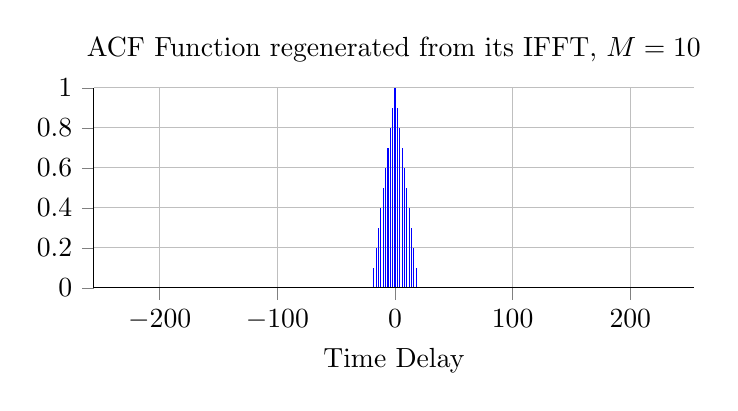
\begin{tikzpicture}

\begin{axis}[%
width=3in,
height=1in,
scale only axis,
every outer y axis line/.append style={black},
every y tick label/.append style={font=\color{black}},
every outer x axis line/.append style={black},
every x tick label/.append style={font=\color{black}},
tick align = outside,
xmin=-256,
xmax=254,
xlabel={Time Delay},
xmajorgrids,
ymin=-1.66533453693773e-16,
ymax=1,
ymajorgrids,
title={ACF Function regenerated from its IFFT, $M = 10$},
axis x line*=bottom,
axis y line*=left
]
\addplot[ycomb,color=blue,solid] plot table[row sep=crcr] {-256	0\\
-254	-5.55111512312578e-17\\
-252	0\\
-250	-1.11022302462516e-16\\
-248	0\\
-246	-2.77555756156289e-17\\
-244	2.77555756156289e-17\\
-242	-5.55111512312578e-17\\
-240	5.55111512312578e-17\\
-238	0\\
-236	3.95668492650429e-17\\
-234	-1.37938759474244e-17\\
-232	-1.14219697790224e-17\\
-230	-7.25273686801708e-18\\
-228	1.01871849571618e-17\\
-226	1.84152327190131e-18\\
-224	1.06215989438577e-17\\
-222	-2.13224799479039e-18\\
-220	7.06757423684502e-18\\
-218	-8.47681591565732e-18\\
-216	1.82198086542736e-17\\
-214	-2.01110946009403e-17\\
-212	3.46944695195361e-18\\
-210	-2.25514051876985e-17\\
-208	-3.46944695195361e-18\\
-206	0\\
-204	-1.38777878078145e-17\\
-202	-5.55111512312578e-17\\
-200	-6.93889390390723e-18\\
-198	5.55111512312578e-17\\
-196	-5.55111512312578e-17\\
-194	-1.38777878078145e-17\\
-192	-1.96261557335472e-17\\
-190	-5.31300992749088e-17\\
-188	-5.88784672006416e-17\\
-186	2.77555756156289e-17\\
-184	-9.81307786677359e-17\\
-182	2.65650496374544e-17\\
-180	-4.33170214081352e-17\\
-178	4.06470994104086e-18\\
-176	-5.02559153120425e-17\\
-174	7.41087389136513e-18\\
-172	-9.10033898610621e-18\\
-170	2.96965249364475e-17\\
-168	-3.8808481089701e-17\\
-166	-2.05594968908316e-17\\
-164	-9.98725574514103e-18\\
-162	1.23915982857246e-17\\
-160	-2.56428082243489e-17\\
-158	3.53476601488415e-18\\
-156	-3.00238655961497e-17\\
-154	-9.34514969325883e-18\\
-152	-4.06802285564554e-17\\
-150	6.51093426476955e-18\\
-148	-1.22391161698259e-17\\
-146	6.93889390390723e-18\\
-144	-6.93889390390723e-18\\
-142	1.38777878078145e-17\\
-140	5.55111512312578e-17\\
-138	0\\
-136	-2.77555756156289e-17\\
-134	0\\
-132	0\\
-130	-2.77555756156289e-17\\
-128	0\\
-126	-2.77555756156289e-17\\
-124	0\\
-122	0\\
-120	0\\
-118	2.77555756156289e-17\\
-116	2.77555756156289e-17\\
-114	-4.16333634234434e-17\\
-112	-6.93889390390723e-18\\
-110	-2.08166817117217e-17\\
-108	-2.07277285422346e-17\\
-106	9.18391977016832e-18\\
-104	-1.32371157563497e-17\\
-102	1.31785882760017e-17\\
-100	7.28174525052325e-18\\
-98	1.92515680565564e-17\\
-96	2.56428082243489e-17\\
-94	1.73422454209975e-17\\
-92	2.04732204102242e-17\\
-90	7.4200128603247e-17\\
-88	-3.19785165847904e-18\\
-86	3.75780620828621e-17\\
-84	3.46944695195361e-18\\
-82	4.68375338513738e-17\\
-80	-6.93889390390723e-18\\
-78	4.5102810375397e-17\\
-76	1.38777878078145e-17\\
-74	5.55111512312578e-17\\
-72	5.55111512312578e-17\\
-70	2.08166817117217e-17\\
-68	0\\
-66	-1.38777878078145e-17\\
-64	1.96261557335472e-17\\
-62	2.53745236592799e-17\\
-60	5.88784672006416e-17\\
-58	2.77555756156289e-17\\
-56	5.88784672006416e-17\\
-54	-1.268726182964e-17\\
-52	-2.36908656745881e-17\\
-50	2.36908656745881e-17\\
-48	-6.93889390390723e-18\\
-46	2.78788586172583e-17\\
-44	8.05559261243773e-18\\
-42	2.92865387256775e-17\\
-40	-1.78468393295369e-17\\
-38	-3.5040871027333e-18\\
-36	4.8175141397701e-17\\
-34	3.65706271294544e-17\\
-32	-1.06215989438577e-17\\
-30	1.43681718940592e-17\\
-28	2.49655940531126e-18\\
-26	-4.19887693173595e-18\\
-24	-4.04962494724488e-18\\
-22	-1.16078772582176e-17\\
-20	-2.70131952972685e-17\\
-18	0.1\\
-16	0.2\\
-14	0.3\\
-12	0.4\\
-10	0.5\\
-8	0.6\\
-6	0.7\\
-4	0.8\\
-2	0.9\\
0	1\\
2	0.9\\
4	0.8\\
6	0.7\\
8	0.6\\
10	0.5\\
12	0.4\\
14	0.3\\
16	0.2\\
18	0.1\\
20	-1.5088616925391e-17\\
22	1.81341300533454e-17\\
24	-4.04962494724487e-18\\
26	-1.89168262938656e-17\\
28	4.32927122891201e-18\\
30	3.86523313685396e-17\\
32	-1.06215989438577e-17\\
34	1.34393451791955e-17\\
36	4.52348460513423e-17\\
38	1.20211177056957e-17\\
40	-1.78468393295369e-17\\
42	1.11708395347706e-18\\
44	1.04083408558608e-17\\
46	3.29597460435593e-17\\
48	3.46944695195361e-18\\
50	1.38777878078145e-17\\
52	-1.38777878078145e-17\\
54	0\\
56	6.93889390390723e-18\\
58	0\\
60	5.55111512312578e-17\\
62	-1.38777878078145e-17\\
64	1.96261557335472e-17\\
66	2.53745236592799e-17\\
68	5.88784672006416e-17\\
70	2.77555756156289e-17\\
72	9.81307786677359e-17\\
74	-1.268726182964e-17\\
76	1.55614457925063e-17\\
78	2.36908656745881e-17\\
80	8.6225518885991e-18\\
82	5.15697242918463e-17\\
84	-3.98354878782849e-18\\
86	6.38905951780185e-17\\
88	-3.19785165847904e-18\\
90	6.3852728952167e-17\\
92	2.70737744960259e-17\\
94	2.83430088091745e-17\\
96	2.56428082243489e-17\\
98	8.01308362397917e-18\\
100	1.62962160226141e-18\\
102	2.68410954752575e-17\\
104	-1.32371157563497e-17\\
106	-1.95248057505745e-17\\
108	-1.22391161698259e-17\\
110	-3.46944695195361e-17\\
112	-1.38777878078145e-17\\
114	-2.77555756156289e-17\\
116	0\\
118	0\\
120	-5.55111512312578e-17\\
122	0\\
124	0\\
126	-5.55111512312578e-17\\
128	0\\
130	-2.77555756156289e-17\\
132	0\\
134	0\\
136	-5.55111512312578e-17\\
138	2.77555756156289e-17\\
140	2.77555756156289e-17\\
142	1.38777878078145e-17\\
144	-6.93889390390723e-18\\
146	2.08166817117217e-17\\
148	-3.75050379741718e-18\\
150	1.42314017395397e-17\\
152	-4.06802285564554e-17\\
154	-1.12951537777943e-17\\
156	-3.56759892444115e-17\\
158	1.65824102459822e-17\\
160	-2.56428082243489e-17\\
162	-8.93766989773709e-19\\
164	-3.38670165933924e-18\\
166	-1.52943852581203e-17\\
168	-3.8808481089701e-17\\
170	1.9579865036091e-17\\
172	-1.73472347597681e-17\\
174	-8.67361737988404e-18\\
176	-4.85722573273506e-17\\
178	-3.12250225675825e-17\\
180	-4.16333634234434e-17\\
182	-5.55111512312578e-17\\
184	-5.55111512312578e-17\\
186	3.46944695195361e-17\\
188	0\\
190	-1.38777878078145e-17\\
192	-1.96261557335472e-17\\
194	-5.31300992749088e-17\\
196	-5.88784672006416e-17\\
198	2.77555756156289e-17\\
200	-5.88784672006416e-17\\
202	2.65650496374544e-17\\
204	-4.06470994104086e-18\\
206	4.06470994104086e-18\\
208	-6.93889390390723e-18\\
210	3.34616395032427e-18\\
212	5.02829516149697e-18\\
214	-1.18513563776278e-17\\
216	1.82198086542736e-17\\
218	-8.56412239101958e-18\\
220	4.12727889048633e-18\\
222	-9.77401281373991e-19\\
224	1.06215989438577e-17\\
226	1.83955408270644e-18\\
228	1.20198967807625e-17\\
230	-6.35817494635547e-18\\
232	-1.14219697790224e-17\\
234	-2.04810616313745e-17\\
236	5.14914276369203e-17\\
238	-3.46944695195361e-17\\
240	2.08166817117217e-17\\
242	1.38777878078145e-17\\
244	-5.55111512312578e-17\\
246	-1.11022302462516e-16\\
248	2.77555756156289e-17\\
250	-1.11022302462516e-16\\
252	-1.66533453693773e-16\\
254	-8.32667268468867e-17\\
};
\addplot [color=black,solid,forget plot]
  table[row sep=crcr]{-256	0\\
254	0\\
};
\end{axis}
\end{tikzpicture}%}
		\label{fig:1_2_d_ifft_10}
	\end{subfigure}
	~ %add desired spacing between images, e. g. ~, \quad, \qquad, \hfill etc.
	\begin{subfigure}[b]{0.49\textwidth}
		\resizebox{\textwidth}{!}{% This file was created by matlab2tikz v0.4.7 (commit 6519689aa9dc12b7be17fdbac3b670671ea448dc) running on MATLAB 8.3.
% Copyright (c) 2008--2014, Nico Schlömer <nico.schloemer@gmail.com>
% All rights reserved.
% Minimal pgfplots version: 1.3
% 
% The latest updates can be retrieved from
%   http://www.mathworks.com/matlabcentral/fileexchange/22022-matlab2tikz
% where you can also make suggestions and rate matlab2tikz.
% 
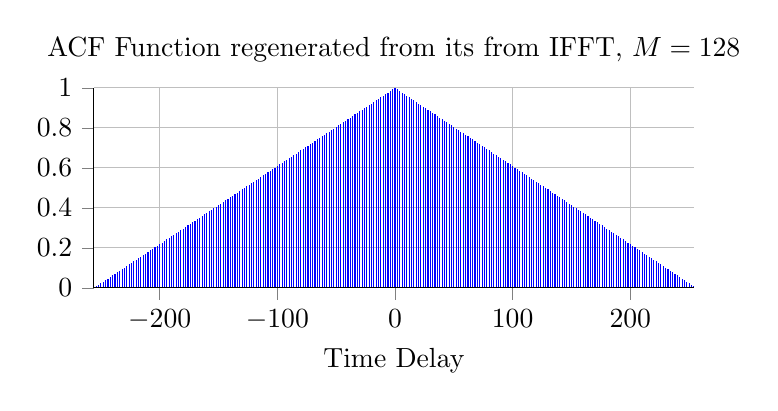
\begin{tikzpicture}

\begin{axis}[%
width=3in,
height=1in,
scale only axis,
every outer y axis line/.append style={black},
every y tick label/.append style={font=\color{black}},
every outer x axis line/.append style={black},
every x tick label/.append style={font=\color{black}},
tick align = outside,
xmin=-256,
xmax=254,
xlabel={Time Delay},
xmajorgrids,
ymin=0,
ymax=1,
ymajorgrids,
title={ACF Function regenerated from its from IFFT, $M = 128$},
axis x line*=bottom,
axis y line*=left
]
\addplot[ycomb,color=blue,solid] plot table[row sep=crcr] {-256	1.11022302462516e-16\\
-254	0.0078125\\
-252	0.0156250000000001\\
-250	0.0234375\\
-248	0.03125\\
-246	0.0390625000000001\\
-244	0.046875\\
-242	0.0546875\\
-240	0.0625000000000001\\
-238	0.0703125\\
-236	0.0781250000000001\\
-234	0.0859375\\
-232	0.0937500000000001\\
-230	0.1015625\\
-228	0.109375\\
-226	0.1171875\\
-224	0.125\\
-222	0.1328125\\
-220	0.140625\\
-218	0.1484375\\
-216	0.15625\\
-214	0.1640625\\
-212	0.171875\\
-210	0.1796875\\
-208	0.1875\\
-206	0.1953125\\
-204	0.203125\\
-202	0.2109375\\
-200	0.21875\\
-198	0.2265625\\
-196	0.234375\\
-194	0.2421875\\
-192	0.25\\
-190	0.2578125\\
-188	0.265625\\
-186	0.2734375\\
-184	0.28125\\
-182	0.2890625\\
-180	0.296875\\
-178	0.3046875\\
-176	0.3125\\
-174	0.3203125\\
-172	0.328125\\
-170	0.3359375\\
-168	0.34375\\
-166	0.3515625\\
-164	0.359375\\
-162	0.3671875\\
-160	0.375\\
-158	0.3828125\\
-156	0.390625\\
-154	0.3984375\\
-152	0.40625\\
-150	0.4140625\\
-148	0.421875\\
-146	0.4296875\\
-144	0.4375\\
-142	0.4453125\\
-140	0.453125\\
-138	0.4609375\\
-136	0.46875\\
-134	0.4765625\\
-132	0.484375\\
-130	0.4921875\\
-128	0.5\\
-126	0.5078125\\
-124	0.515625\\
-122	0.5234375\\
-120	0.53125\\
-118	0.5390625\\
-116	0.546875\\
-114	0.5546875\\
-112	0.5625\\
-110	0.5703125\\
-108	0.578125\\
-106	0.5859375\\
-104	0.59375\\
-102	0.6015625\\
-100	0.609375\\
-98	0.6171875\\
-96	0.625\\
-94	0.6328125\\
-92	0.640625\\
-90	0.6484375\\
-88	0.65625\\
-86	0.6640625\\
-84	0.671875\\
-82	0.6796875\\
-80	0.6875\\
-78	0.6953125\\
-76	0.703125\\
-74	0.7109375\\
-72	0.71875\\
-70	0.7265625\\
-68	0.734375\\
-66	0.7421875\\
-64	0.75\\
-62	0.7578125\\
-60	0.765625\\
-58	0.7734375\\
-56	0.78125\\
-54	0.7890625\\
-52	0.796875\\
-50	0.8046875\\
-48	0.8125\\
-46	0.8203125\\
-44	0.828125\\
-42	0.8359375\\
-40	0.84375\\
-38	0.8515625\\
-36	0.859375\\
-34	0.8671875\\
-32	0.875\\
-30	0.8828125\\
-28	0.890625\\
-26	0.8984375\\
-24	0.90625\\
-22	0.9140625\\
-20	0.921875\\
-18	0.9296875\\
-16	0.9375\\
-14	0.9453125\\
-12	0.953125\\
-10	0.9609375\\
-8	0.96875\\
-6	0.9765625\\
-4	0.984375\\
-2	0.9921875\\
0	1\\
2	0.9921875\\
4	0.984375\\
6	0.9765625\\
8	0.96875\\
10	0.9609375\\
12	0.953125\\
14	0.9453125\\
16	0.9375\\
18	0.9296875\\
20	0.921875\\
22	0.9140625\\
24	0.90625\\
26	0.8984375\\
28	0.890625\\
30	0.8828125\\
32	0.875\\
34	0.8671875\\
36	0.859375\\
38	0.8515625\\
40	0.84375\\
42	0.8359375\\
44	0.828125\\
46	0.8203125\\
48	0.8125\\
50	0.8046875\\
52	0.796875\\
54	0.7890625\\
56	0.78125\\
58	0.7734375\\
60	0.765625\\
62	0.7578125\\
64	0.75\\
66	0.7421875\\
68	0.734375\\
70	0.7265625\\
72	0.71875\\
74	0.7109375\\
76	0.703125\\
78	0.6953125\\
80	0.6875\\
82	0.6796875\\
84	0.671875\\
86	0.6640625\\
88	0.65625\\
90	0.6484375\\
92	0.640625\\
94	0.6328125\\
96	0.625\\
98	0.6171875\\
100	0.609375\\
102	0.6015625\\
104	0.59375\\
106	0.5859375\\
108	0.578125\\
110	0.5703125\\
112	0.5625\\
114	0.5546875\\
116	0.546875\\
118	0.5390625\\
120	0.53125\\
122	0.5234375\\
124	0.515625\\
126	0.5078125\\
128	0.5\\
130	0.4921875\\
132	0.484375\\
134	0.4765625\\
136	0.46875\\
138	0.4609375\\
140	0.453125\\
142	0.4453125\\
144	0.4375\\
146	0.4296875\\
148	0.421875\\
150	0.4140625\\
152	0.40625\\
154	0.3984375\\
156	0.390625\\
158	0.3828125\\
160	0.375\\
162	0.3671875\\
164	0.359375\\
166	0.3515625\\
168	0.34375\\
170	0.3359375\\
172	0.328125\\
174	0.3203125\\
176	0.3125\\
178	0.3046875\\
180	0.296875\\
182	0.2890625\\
184	0.28125\\
186	0.2734375\\
188	0.265625\\
190	0.2578125\\
192	0.25\\
194	0.2421875\\
196	0.234375\\
198	0.2265625\\
200	0.21875\\
202	0.2109375\\
204	0.203125\\
206	0.1953125\\
208	0.1875\\
210	0.1796875\\
212	0.171875\\
214	0.1640625\\
216	0.15625\\
218	0.1484375\\
220	0.140625\\
222	0.1328125\\
224	0.125\\
226	0.1171875\\
228	0.109375\\
230	0.1015625\\
232	0.0937500000000001\\
234	0.0859374999999999\\
236	0.078125\\
238	0.0703124999999999\\
240	0.0625\\
242	0.0546875\\
244	0.0468749999999999\\
246	0.0390625\\
248	0.03125\\
250	0.0234374999999999\\
252	0.0156250000000001\\
254	0.00781249999999989\\
};
\addplot [color=black,solid,forget plot]
  table[row sep=crcr]{-256	0\\
254	0\\
};
\end{axis}
\end{tikzpicture}%}
		\label{fig:1_2_d_ifft_128}
	\end{subfigure}
	\label{fig:1_2_d_ifft}
	\caption{\textit{Shifted IFFTs of the PSD}}
\end{figure}


\begin{figure}[h]
	\centering
	\begin{subfigure}[b]{0.49\textwidth}
		\resizebox{\textwidth}{!}{% This file was created by matlab2tikz v0.4.7 (commit 6519689aa9dc12b7be17fdbac3b670671ea448dc) running on MATLAB 8.3.
% Copyright (c) 2008--2014, Nico Schlömer <nico.schloemer@gmail.com>
% All rights reserved.
% Minimal pgfplots version: 1.3
% 
% The latest updates can be retrieved from
%   http://www.mathworks.com/matlabcentral/fileexchange/22022-matlab2tikz
% where you can also make suggestions and rate matlab2tikz.
% 
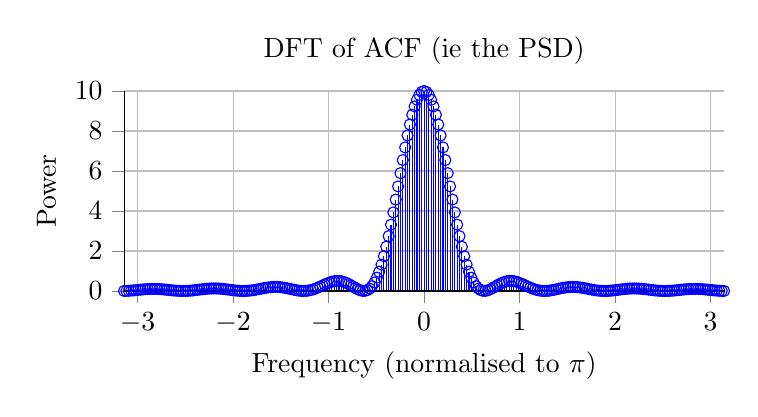
\begin{tikzpicture}

\begin{axis}[%
width=3in,
height=1in,
scale only axis,
every outer y axis line/.append style={black},
every y tick label/.append style={font=\color{black}},
every outer x axis line/.append style={black},
every x tick label/.append style={font=\color{black}},
tick align = outside,
xmin=-3.14159265358979,
xmax=3.14159265358979,
xlabel={Frequency (normalised to $ \pi $)},
xmajorgrids,
ymin=0,
ymax=10,
ylabel={Power},
ymajorgrids,
title={DFT of ACF (ie the PSD)},
axis x line*=bottom,
axis y line*=left
]
\addplot[ycomb,color=blue,solid,mark=o,mark options={solid}] plot table[row sep=crcr] {-3.14159265358979	0.000378988897115282\\
-3.11685570356153	0.0033775418587593\\
-3.09211875353326	0.00919887800597178\\
-3.06738180350499	0.0175016060124896\\
-3.04264485347673	0.0277984354043452\\
-3.01790790344846	0.0394843568772002\\
-2.9931709534202	0.0518716839950063\\
-2.96843400339193	0.0642299681359829\\
-2.94369705336366	0.0758285175203089\\
-2.9189601033354	0.0859790965550988\\
-2.89422315330713	0.0940763625190739\\
-2.86948620327887	0.0996337143174552\\
-2.8447492532506	0.102312476678775\\
-2.82001230322233	0.101942709525753\\
-2.79527535319407	0.0985343965838238\\
-2.7705384031658	0.0922783043556371\\
-2.74580145313754	0.0835363830084124\\
-2.72106450310927	0.0728221725495515\\
-2.696327553081	0.060772248120425\\
-2.67159060305274	0.0481102554752904\\
-2.64685365302447	0.0356055225693278\\
-2.62211670299621	0.0240285607835518\\
-2.59737975296794	0.0141059704690513\\
-2.57264280293967	0.00647732777372036\\
-2.54790585291141	0.00165654820388524\\
-2.52316890288314	0\\
-2.49843195285487	0.00168328786448976\\
-2.47369500282661	0.00668816283073246\\
-2.44895805279834	0.0148004614348181\\
-2.42422110277008	0.0256193662967289\\
-2.39948415274181	0.0385776437696065\\
-2.37474720271354	0.052971887345538\\
-2.35001025268528	0.0680012128537339\\
-2.32527330265701	0.0828123460726914\\
-2.30053635262875	0.0965486443934246\\
-2.27579940260048	0.108400325444963\\
-2.25106245257221	0.117653054223245\\
-2.22632550254395	0.123732075587978\\
-2.20158855251568	0.126239271959526\\
-2.17685160248742	0.124980869033386\\
-2.15211465245915	0.119983989397236\\
-2.12737770243088	0.111500841551587\\
-2.10264075240262	0.0999999999999999\\
-2.07790380237435	0.086144945815086\\
-2.05316685234609	0.0707607582393038\\
-2.02842990231782	0.0547905370763618\\
-2.00369295228955	0.0392437543816701\\
-1.97895600226129	0.0251392467364777\\
-1.95421905223302	0.0134459355746087\\
-1.92948210220475	0.00502457866213267\\
-1.90474515217649	0.000573895024344543\\
-1.88000820214822	0.000584261587985141\\
-1.85527125211996	0.00530185544543615\\
-1.83053430209169	0.014705623577935\\
-1.80579735206342	0.0284988240259788\\
-1.78106040203516	0.0461161291654325\\
-1.75632345200689	0.0667464502129547\\
-1.73158650197863	0.0893707748097577\\
-1.70684955195036	0.112813452075412\\
-1.68211260192209	0.135804558224093\\
-1.65737565189383	0.157050275415477\\
-1.63263870186556	0.175307657695964\\
-1.6079017518373	0.189459775172247\\
-1.58316480180903	0.19858704725956\\
-1.55842785178076	0.202030614492431\\
-1.5336909017525	0.199443861598004\\
-1.50895395172423	0.190828686420805\\
-1.48421700169597	0.176553792421701\\
-1.4594800516677	0.157353138435747\\
-1.43474310163943	0.134303669888549\\
-1.41000615161117	0.108782534261852\\
-1.3852692015829	0.082405097700833\\
-1.36053225155463	0.0569461730898774\\
-1.33579530152637	0.034247885623577\\
-1.3110583514981	0.0161184847506591\\
-1.28632140146984	0.00422711102974243\\
-1.26158445144157	0\\
-1.2368475014133	0.00452381952891347\\
-1.21211055138504	0.0184617708889252\\
-1.18737360135677	0.0419877288354474\\
-1.16263665132851	0.0747430579888372\\
-1.13789970130024	0.115819841771999\\
-1.11316275127197	0.163773129531353\\
-1.08842580124371	0.216663493172725\\
-1.06368885121544	0.272129743129657\\
-1.03895190118718	0.327490149361259\\
-1.01421495115891	0.379869016264924\\
-0.989478001130644	0.426344042922973\\
-0.964741051102378	0.464108632771142\\
-0.940004101074111	0.490642265728266\\
-0.915267151045845	0.50388126930035\\
-0.890530201017579	0.5023818705269\\
-0.865793250989313	0.485467311812398\\
-0.841056300961047	0.453351089229754\\
-0.816319350932781	0.407229023652982\\
-0.791582400904515	0.349333887684378\\
-0.766845450876249	0.282947652385176\\
-0.742108500847983	0.212368038908085\\
-0.717371550819716	0.142827898674447\\
-0.69263460079145	0.0803679274265149\\
-0.667897650763184	0.0316652603567495\\
-0.643160700734918	0.00382250949801258\\
-0.618423750706652	0.00412370130732193\\
-0.593686800678386	0.0397652652574135\\
-0.56894985065012	0.117571633279188\\
-0.544212900621854	0.243706065452989\\
-0.519475950593588	0.423387963492397\\
-0.494739000565322	0.660628130819956\\
-0.470002050537056	0.957993165456922\\
-0.44526510050879	1.31640942842425\\
-0.420528150480523	1.73501583502584\\
-0.395791200452257	2.21107310820204\\
-0.371054250423991	2.73993516950041\\
-0.346317300395725	3.31508609778313\\
-0.321580350367459	3.92824364559302\\
-0.296843400339193	4.56952776493921\\
-0.272106450310927	5.22769006070444\\
-0.247369500282661	5.89039766491197\\
-0.222632550254395	6.5445628096979\\
-0.197895600226129	7.17670746461488\\
-0.173158650197863	7.77335087698578\\
-0.148421700169596	8.32140677948926\\
-0.12368475014133	8.80857645596934\\
-0.0989478001130646	9.22372381326993\\
-0.0742108500847984	9.55721910065888\\
-0.0494739000565323	9.80123893393101\\
-0.0247369500282657	9.95001178173265\\
0	10\\
0.0247369500282661	9.95001178173265\\
0.0494739000565323	9.80123893393101\\
0.074210850084798	9.55721910065888\\
0.0989478001130646	9.22372381326993\\
0.123684750141331	8.80857645596934\\
0.148421700169596	8.32140677948926\\
0.173158650197863	7.77335087698578\\
0.197895600226129	7.17670746461488\\
0.222632550254395	6.5445628096979\\
0.247369500282661	5.89039766491197\\
0.272106450310927	5.22769006070444\\
0.296843400339193	4.56952776493921\\
0.321580350367459	3.92824364559302\\
0.346317300395725	3.31508609778313\\
0.371054250423991	2.73993516950041\\
0.395791200452257	2.21107310820204\\
0.420528150480524	1.73501583502584\\
0.445265100508789	1.31640942842425\\
0.470002050537055	0.957993165456922\\
0.494739000565322	0.660628130819956\\
0.519475950593588	0.423387963492397\\
0.544212900621854	0.243706065452989\\
0.56894985065012	0.117571633279188\\
0.593686800678386	0.0397652652574135\\
0.618423750706652	0.00412370130732193\\
0.643160700734918	0.00382250949801258\\
0.667897650763185	0.0316652603567495\\
0.69263460079145	0.0803679274265149\\
0.717371550819716	0.142827898674447\\
0.742108500847983	0.212368038908085\\
0.766845450876249	0.282947652385176\\
0.791582400904515	0.349333887684378\\
0.816319350932781	0.407229023652982\\
0.841056300961047	0.453351089229754\\
0.865793250989313	0.485467311812398\\
0.890530201017579	0.5023818705269\\
0.915267151045845	0.50388126930035\\
0.940004101074111	0.490642265728266\\
0.964741051102378	0.464108632771142\\
0.989478001130644	0.426344042922973\\
1.01421495115891	0.379869016264924\\
1.03895190118718	0.327490149361259\\
1.06368885121544	0.272129743129657\\
1.08842580124371	0.216663493172725\\
1.11316275127197	0.163773129531353\\
1.13789970130024	0.115819841771999\\
1.16263665132851	0.0747430579888372\\
1.18737360135677	0.0419877288354474\\
1.21211055138504	0.0184617708889252\\
1.2368475014133	0.00452381952891347\\
1.26158445144157	0\\
1.28632140146984	0.00422711102974243\\
1.3110583514981	0.0161184847506591\\
1.33579530152637	0.034247885623577\\
1.36053225155464	0.0569461730898774\\
1.3852692015829	0.082405097700833\\
1.41000615161117	0.108782534261852\\
1.43474310163943	0.134303669888549\\
1.4594800516677	0.157353138435747\\
1.48421700169597	0.176553792421701\\
1.50895395172423	0.190828686420805\\
1.5336909017525	0.199443861598004\\
1.55842785178076	0.202030614492431\\
1.58316480180903	0.19858704725956\\
1.6079017518373	0.189459775172247\\
1.63263870186556	0.175307657695964\\
1.65737565189383	0.157050275415477\\
1.68211260192209	0.135804558224093\\
1.70684955195036	0.112813452075412\\
1.73158650197863	0.0893707748097577\\
1.75632345200689	0.0667464502129547\\
1.78106040203516	0.0461161291654325\\
1.80579735206342	0.0284988240259788\\
1.83053430209169	0.014705623577935\\
1.85527125211996	0.00530185544543615\\
1.88000820214822	0.000584261587985141\\
1.90474515217649	0.000573895024344543\\
1.92948210220476	0.00502457866213267\\
1.95421905223302	0.0134459355746087\\
1.97895600226129	0.0251392467364777\\
2.00369295228955	0.0392437543816701\\
2.02842990231782	0.0547905370763618\\
2.05316685234609	0.0707607582393038\\
2.07790380237435	0.086144945815086\\
2.10264075240262	0.0999999999999999\\
2.12737770243088	0.111500841551587\\
2.15211465245915	0.119983989397236\\
2.17685160248742	0.124980869033386\\
2.20158855251568	0.126239271959526\\
2.22632550254395	0.123732075587978\\
2.25106245257221	0.117653054223245\\
2.27579940260048	0.108400325444963\\
2.30053635262875	0.0965486443934246\\
2.32527330265701	0.0828123460726914\\
2.35001025268528	0.0680012128537339\\
2.37474720271354	0.052971887345538\\
2.39948415274181	0.0385776437696065\\
2.42422110277008	0.0256193662967289\\
2.44895805279834	0.0148004614348181\\
2.47369500282661	0.00668816283073246\\
2.49843195285487	0.00168328786448976\\
2.52316890288314	0\\
2.54790585291141	0.00165654820388524\\
2.57264280293967	0.00647732777372036\\
2.59737975296794	0.0141059704690513\\
2.62211670299621	0.0240285607835518\\
2.64685365302447	0.0356055225693278\\
2.67159060305274	0.0481102554752904\\
2.696327553081	0.060772248120425\\
2.72106450310927	0.0728221725495515\\
2.74580145313754	0.0835363830084124\\
2.7705384031658	0.0922783043556371\\
2.79527535319407	0.0985343965838238\\
2.82001230322233	0.101942709525753\\
2.8447492532506	0.102312476678775\\
2.86948620327887	0.0996337143174552\\
2.89422315330713	0.0940763625190739\\
2.9189601033354	0.0859790965550988\\
2.94369705336366	0.0758285175203089\\
2.96843400339193	0.0642299681359829\\
2.9931709534202	0.0518716839950063\\
3.01790790344846	0.0394843568772002\\
3.04264485347673	0.0277984354043452\\
3.067381803505	0.0175016060124896\\
3.09211875353326	0.00919887800597178\\
3.11685570356153	0.0033775418587593\\
3.14159265358979	0.000378988897115282\\
};
\addplot [color=black,solid,forget plot]
  table[row sep=crcr]{-3.14159265358979	0\\
3.14159265358979	0\\
};
\end{axis}
\end{tikzpicture}%}
		\label{fig:1_2_d_dft_odd}
	\end{subfigure}
	~ %add desired spacing between images, e. g. ~, \quad, \qquad, \hfill etc.
	\begin{subfigure}[b]{0.49\textwidth}
		\resizebox{\textwidth}{!}{% This file was created by matlab2tikz v0.4.7 (commit 6519689aa9dc12b7be17fdbac3b670671ea448dc) running on MATLAB 8.3.
% Copyright (c) 2008--2014, Nico Schlömer <nico.schloemer@gmail.com>
% All rights reserved.
% Minimal pgfplots version: 1.3
% 
% The latest updates can be retrieved from
%   http://www.mathworks.com/matlabcentral/fileexchange/22022-matlab2tikz
% where you can also make suggestions and rate matlab2tikz.
% 
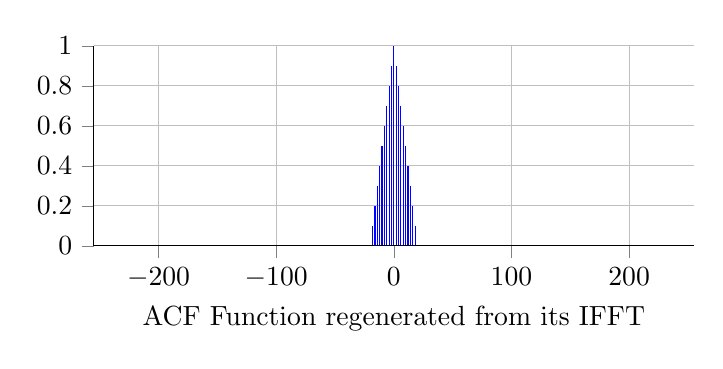
\begin{tikzpicture}

\begin{axis}[%
width=3in,
height=1in,
scale only axis,
every outer y axis line/.append style={black},
every y tick label/.append style={font=\color{black}},
every outer x axis line/.append style={black},
every x tick label/.append style={font=\color{black}},
tick align = outside,
xmin=-255,
xmax=255,
xlabel={ACF Function regenerated from its IFFT},
xmajorgrids,
ymin=-1.28872947172175e-16,
ymax=1,
ymajorgrids,
axis x line*=bottom,
axis y line*=left
]
\addplot[ycomb,color=blue,solid] plot table[row sep=crcr] {-255	7.7715611723761e-17\\
-252.992125984252	7.05318156820688e-17\\
-250.984251968504	2.96059473233375e-17\\
-248.976377952756	-8.7076315656875e-18\\
-246.968503937008	8.44640261871688e-17\\
-244.96062992126	4.876273676785e-17\\
-242.952755905512	5.05042630809875e-17\\
-240.944881889764	1.21906841919625e-17\\
-238.937007874016	-2.8351528320931e-17\\
-236.929133858268	3.56169627867612e-17\\
-234.92125984252	3.42169464857515e-17\\
-232.913385826772	-3.09478576051832e-17\\
-230.905511811024	-1.1607312212628e-17\\
-228.897637795276	2.91705657450531e-17\\
-226.889763779528	7.40148683083438e-18\\
-224.88188976378	2.37282960164984e-17\\
-222.874015748032	3.91843420455938e-17\\
-220.866141732283	-4.00551052021625e-17\\
-218.858267716535	-2.26398420707875e-17\\
-216.850393700787	-1.07103868257956e-16\\
-214.842519685039	-1.39322105051e-17\\
-212.834645669291	8.7076315656875e-18\\
-210.826771653543	1.39322105051e-17\\
-208.818897637795	-4.04811221541714e-17\\
-206.811023622047	-1.6004087206344e-17\\
-204.803149606299	2.36199307405631e-17\\
-202.795275590551	8.91325526598358e-18\\
-200.787401574803	-3.00745264726524e-17\\
-198.779527559055	1.34968289268156e-17\\
-196.771653543307	3.65720525758875e-17\\
-194.763779527559	4.35381578284375e-18\\
-192.755905511811	2.089831575765e-17\\
-190.748031496063	-7.48856314649125e-17\\
-188.740157480315	-6.96610525255e-18\\
-186.732283464567	-1.21906841919625e-17\\
-184.724409448819	-7.3144105151775e-17\\
-182.716535433071	-1.28872947172175e-16\\
-180.708661417323	1.23565854005466e-33\\
-178.700787401575	6.4571838634985e-18\\
-176.692913385827	-9.08297443659701e-18\\
-174.685039370079	-4.53102514630706e-17\\
-172.677165354331	-3.23159277371556e-17\\
-170.669291338583	2.11755987350095e-17\\
-168.661417322835	-1.71975723422328e-17\\
-166.653543307087	-3.8313578889025e-17\\
-164.645669291339	-3.39597631061813e-17\\
-162.637795275591	3.483052626275e-17\\
-160.629921259843	4.00551052021625e-17\\
-158.622047244094	4.35381578284375e-17\\
-156.614173228346	4.5279684141575e-17\\
-154.606299212598	2.78644210102e-17\\
-152.59842519685	1.01008526161975e-16\\
-150.590551181102	6.05990820619268e-34\\
-148.582677165354	-9.01091078859765e-18\\
-146.574803149606	1.56744935689931e-17\\
-144.566929133858	2.89436811815596e-17\\
-142.55905511811	-3.76030608197455e-17\\
-140.551181102362	-4.09902409396081e-17\\
-138.543307086614	-2.67759670644891e-17\\
-136.535433070866	2.13336973359344e-17\\
-134.527559055118	-1.65444999748063e-17\\
-132.51968503937	-6.44364735860875e-17\\
-130.511811023622	-1.7415263131375e-18\\
-128.503937007874	1.0449157878825e-17\\
-126.496062992126	2.96059473233375e-17\\
-124.488188976378	-3.483052626275e-17\\
-122.48031496063	-3.483052626275e-17\\
-120.472440944882	2.78644210102e-17\\
-118.464566929134	-1.96483819024605e-17\\
-116.456692913386	6.29768317846262e-18\\
-114.448818897638	-2.41200988892177e-17\\
-112.44094488189	-3.05109161921111e-17\\
-110.433070866142	6.17981417531474e-17\\
-108.425196850394	-2.98236381124797e-17\\
-106.417322834646	-1.48029736616688e-17\\
-104.409448818898	-1.65444999748063e-17\\
-102.40157480315	-6.09534209598125e-18\\
-100.393700787402	1.56737368182375e-17\\
-98.3858267716535	2.96059473233375e-17\\
-96.3779527559055	1.7415263131375e-17\\
-94.3700787401575	5.05042630809875e-17\\
-92.3622047244095	6.6177999899225e-17\\
-90.3543307086614	2.78644210102e-17\\
-88.3464566929134	4.78942245800454e-17\\
-86.3385826771654	-7.6349435453089e-19\\
-84.3307086614173	1.14244779436616e-17\\
-82.3228346456693	1.19742969718424e-17\\
-80.3149606299213	9.51477804116804e-18\\
-78.3070866141732	6.53072367426563e-19\\
-76.2992125984252	2.61228946970625e-17\\
-74.2913385826772	-8.7076315656875e-19\\
-72.2834645669291	-9.57839472225625e-18\\
-70.2755905511811	3.1347473636475e-17\\
-68.2677165354331	1.7415263131375e-17\\
-66.259842519685	8.7076315656875e-18\\
-64.251968503937	8.7076315656875e-18\\
-62.244094488189	-1.7415263131375e-17\\
-60.2362204724409	-1.33243125173277e-33\\
-58.2283464566929	-3.67005967126425e-17\\
-56.2204724409449	-3.6926398077842e-17\\
-54.2125984251969	2.84249385333243e-17\\
-52.2047244094488	-1.69778679330413e-17\\
-50.1968503937008	-2.20368539965845e-17\\
-48.1889763779528	-3.67897433650297e-17\\
-46.1811023622047	-5.68172959661109e-17\\
-44.1732283464567	-2.65582762753469e-17\\
-42.1653543307087	-4.13612499370156e-17\\
-40.1574803149606	1.30614473485313e-18\\
-38.1496062992126	-1.82860262879438e-17\\
-36.1417322834646	1.82860262879438e-17\\
-34.1338582677165	-6.09534209598125e-18\\
-32.1259842519685	1.56737368182375e-17\\
-30.1181102362205	7.01500172555039e-34\\
-28.1102362204724	7.18303901000423e-17\\
-26.1023622047244	-1.62528733472875e-17\\
-24.0944881889764	1.57541604617689e-17\\
-22.0866141732284	-6.80244605438659e-18\\
-20.0787401574803	3.36002436284521e-17\\
-18.0708661417323	0.1\\
-16.0629921259843	0.2\\
-14.0551181102362	0.3\\
-12.0472440944882	0.4\\
-10.0393700787401	0.5\\
-8.03149606299212	0.6\\
-6.02362204724409	0.7\\
-4.01574803149606	0.8\\
-2.00787401574803	0.9\\
0	1\\
2.00787401574803	0.9\\
4.01574803149606	0.8\\
6.02362204724409	0.7\\
8.03149606299212	0.6\\
10.0393700787401	0.5\\
12.0472440944882	0.4\\
14.0551181102362	0.3\\
16.0629921259842	0.2\\
18.0708661417323	0.1\\
20.0787401574803	2.089831575765e-17\\
22.0866141732283	6.96610525255e-17\\
24.0944881889764	4.17966315153e-17\\
26.1023622047244	6.96610525255e-17\\
28.1102362204724	-1.39322105051e-17\\
30.1181102362204	-7.01500172555039e-34\\
32.1259842519685	6.74917149509578e-17\\
34.1338582677166	-3.94759686731125e-17\\
36.1417322834646	-1.57541604617689e-17\\
38.1496062992126	-2.10619749558134e-17\\
40.1574803149607	-1.96680331233521e-17\\
42.1653543307087	-1.39322105051e-17\\
44.1732283464567	-2.78644210102e-17\\
46.1811023622047	-5.57288420204e-17\\
48.1889763779528	-5.57288420204e-17\\
50.1968503937008	0\\
52.2047244094488	0\\
54.2125984251969	-1.114576840408e-16\\
56.2204724409449	5.57288420204e-17\\
58.2283464566929	0\\
60.2362204724409	1.33243125173277e-33\\
62.244094488189	-4.68926663179575e-17\\
64.251968503937	-1.8802443942558e-17\\
66.259842519685	2.73039034870757e-17\\
68.2677165354331	1.69778679330413e-17\\
70.2755905511811	8.10464349148445e-18\\
72.2834645669291	-1.89390986553703e-17\\
74.2913385826772	-1.98098618119391e-17\\
76.2992125984252	-1.87214078662281e-17\\
78.3070866141732	-1.43675920833844e-17\\
80.3149606299212	-1.30614473485313e-18\\
82.3228346456693	4.61504472981438e-17\\
84.3307086614173	-1.82860262879438e-17\\
86.3385826771653	6.09534209598125e-18\\
88.3464566929134	4.00551052021625e-17\\
90.3543307086614	2.78644210102e-17\\
92.3622047244094	6.35634594607546e-17\\
94.3700787401575	7.6349435453089e-19\\
96.3779527559055	1.64399430665384e-17\\
98.3858267716536	2.98223345434576e-17\\
100.393700787402	3.2281853474132e-17\\
102.40157480315	-1.45852828725266e-17\\
104.409448818898	1.91567894445125e-17\\
106.417322834646	-6.09534209598125e-18\\
108.425196850394	-1.13199210353938e-17\\
110.433070866142	5.2245789394125e-17\\
112.44094488189	2.4381368383925e-17\\
114.448818897638	-8.7076315656875e-18\\
116.456692913386	-8.7076315656875e-18\\
118.464566929134	1.7415263131375e-17\\
120.472440944882	2.78644210102e-17\\
122.48031496063	-3.60804601179395e-17\\
124.488188976378	2.15667378317374e-17\\
126.496062992126	-3.74432212098229e-18\\
128.503937007874	-2.52179258282889e-17\\
130.511811023622	7.86291077235266e-18\\
132.51968503937	-1.19729934028203e-17\\
134.527559055118	8.7076315656875e-19\\
136.535433070866	9.57839472225625e-18\\
138.543307086614	-6.35657104295188e-17\\
140.551181102362	-1.7415263131375e-18\\
142.55905511811	-1.56737368182375e-17\\
144.566929133858	2.4381368383925e-17\\
146.574803149606	6.09534209598125e-17\\
148.582677165354	-3.8313578889025e-17\\
150.590551181102	-6.05990820619268e-34\\
152.59842519685	9.01091078859765e-18\\
154.606299212598	2.61221379463069e-17\\
156.614173228346	-1.50114706764596e-17\\
158.622047244094	3.76030608197455e-17\\
160.629921259843	-8.06390575691878e-19\\
162.637795275591	5.87765130683906e-18\\
164.645669291339	4.78919736112813e-18\\
166.653543307087	-3.91843420455938e-17\\
168.661417322835	-3.30889999496125e-17\\
170.669291338583	-1.21906841919625e-17\\
172.677165354331	-8.0110210404325e-17\\
174.685039370079	-5.74703683335375e-17\\
176.692913385827	-4.876273676785e-17\\
178.700787401575	-9.055936828315e-17\\
180.708661417323	-1.23565854005466e-33\\
182.716535433071	-6.4571838634985e-18\\
184.724409448819	9.08297443659701e-18\\
186.732283464567	1.74458304528706e-17\\
188.740157480315	-2.34129142832444e-17\\
190.748031496063	-2.11755987350095e-17\\
192.755905511811	-2.45990591730672e-17\\
194.763779527559	3.65720525758875e-17\\
196.771653543307	1.13199210353938e-17\\
198.779527559055	6.6177999899225e-17\\
200.787401574803	-1.91567894445125e-17\\
202.795275590551	1.91567894445125e-17\\
204.803149606299	-3.483052626275e-18\\
206.811023622047	-1.39322105051e-17\\
208.818897637795	6.6177999899225e-17\\
210.826771653543	1.39322105051e-17\\
212.834645669291	-3.61460356238786e-17\\
214.842519685039	-1.1860333803856e-17\\
216.850393700787	-2.72161498291311e-18\\
218.858267716535	6.07477972595164e-17\\
220.866141732283	-1.17221050426476e-17\\
222.874015748031	2.48167499622094e-17\\
224.88188976378	0\\
226.889763779528	-2.61228946970625e-18\\
228.897637795276	3.483052626275e-17\\
230.905511811024	-1.56737368182375e-17\\
232.913385826772	-6.96610525255e-18\\
234.92125984252	1.21906841919625e-17\\
236.929133858268	3.483052626275e-18\\
238.937007874016	-3.1347473636475e-17\\
240.944881889764	1.21906841919625e-17\\
242.952755905512	-2.0411208446919e-17\\
244.96062992126	4.10101949912888e-17\\
246.968503937008	7.89822638681861e-17\\
248.976377952756	6.22953312416582e-17\\
250.984251968504	4.46963121622405e-17\\
252.992125984252	3.35243815278969e-17\\
255	4.04904867804469e-17\\
};
\addplot [color=black,solid,forget plot]
  table[row sep=crcr]{-255	0\\
255	0\\
};
\end{axis}
\end{tikzpicture}%}
		\label{fig:1_2_d_ifft_odd}
	\end{subfigure}
	\label{fig:1_2_d_ifft}
	\caption{\textit{Odd length DFT and IFFT functions, demonstrating the correct shift to reconstruct the ACF}}
\end{figure}


\end{document}

